%!TEX root = /Users/mpking/Dropbox/writing/king_dissertation/king_dissertation_master.tex
\chapter{Simulation of Electron-Induced SEUs} % (fold)
\label{ch:simulation_of_electron_induced_seus}
The experimental results from Chapter~\ref{cha:experimental_investigation_of_electron_induced_seus} show that 28 and 45~nm SRAMs exhibit SEU sensitivity when exposed to energetic X-rays. 
Data analysis of those results indicates that the observed errors are electron-induced SEUs.
This chapter presents simulations and analysis of Monte Carlo radiation transport codes investigating the experimental results of Chapter~\ref{cha:experimental_investigation_of_electron_induced_seus}.
Section~\ref{sec:simulation_of_x_ray_energy_deposition_in_srams} presents simulations of an X-ray spectrum, consistent with that used in Chapter~\ref{cha:experimental_investigation_of_electron_induced_seus}, incident on a target structure representative of 45~nm bulk SRAMs.
Simulation results are shown to be in good agreement with the experimental data from Chapter~\ref{cha:experimental_investigation_of_electron_induced_seus} and show that photo-electrons generated by incident X-rays deposit energy in excess of the estimated critical charge under a wide range of applied bias.
The relative impact of electron-induced SEUs in the space radiation environment is presented by performing error-rate calculations for a 45~nm SRAM in the geosynchronous orbit and environment during the solar minimum cycle in Section~\ref{sec:electron_induced_seu_event_rates}.
Additional error-rate analysis is performed for the Jovian environment.
Analysis of $\delta$-ray contributions to single- and multiple-bit upset rates for SRAMs irradiated with heavy ions is discussed in Section~\ref{sec:impact_of_delta_rays_on_microelectronics}.

\section{Simulation of X-ray Energy Deposition in SRAMs} % (fold)
\label{sec:simulation_of_x_ray_energy_deposition_in_srams}
Radiation transport simulations were performed with MRED \cite{Weller:2010ud}, a Geant4-based code \cite{Agostinelli:2003vd} with Fortran extensions that include PENELOPE 2008 \cite{Salvat:ue}, to evaluate the potential impact of electrons produced by energetic X-rays on the device SEU response. 
The use of the PENELOPE 2008 package \cite{Salvat:ue} increases the fidelity and resolution of calculations involving low energy (less than 50~keV) electrons, photons and positrons.
PENELOPE 2008 extends the low-energy range for electromagnetic processes from 250 eV down to approximately 100~eV and also tracks electrons with greater spatial resolution. 
These refinements produce increased fidelity of energy deposition estimates in the small sensitive volumes of interest in this work.%

High-energy protons cause single-event effects primarily through secondary ions produced in nuclear reactions \cite{Heidel:2006tp,Heidel:2008vf,Heidel:2009vx,Rodbell:2007vl}. 
For a given proton energy, experimental cross-sections are expressed with reference to the primary proton flux, regardless of the upset mechanism. 
In this sense, the case of single-event effects caused by secondary electrons is analogous. 
Results in this work are therefore plotted as a function of the incident X-ray fluence, which provides the most consistent reference for analyzing SEUs caused by secondary photo-electrons.
The attenuated X-ray energy spectrum from Fig.~\ref{fig:aracor_spectrum} is used in the simulations to simulate the full X-ray exposure environment and range of generated electron energies incident on the exposed SRAM test chip. 
A 4~kbit SRAM array is simulated, using a sensitive volume structure consistent with a 45~nm bulk SRAM using MRED.
Energy deposition is calculated for individual X-rays on an event-by-event basis.
The sensitive volume geometry used was 0.22~$\mu$m$^2$ $\times$ 500~nm, which is representative of 45 nm processes in the ITRS roadmap \cite{itrs:2012}. 
Additionally, the simulated structure includes the 1~mm aluminum attenuator and appropriate BEOL thickness with 15~$\mu$m of oxide and metallization. 
The SRAM was simulated to a total photon fluence of 2$\times$10$^9$~cm$^{-2}$.
This fluence was found to be sufficient to determine the energy deposited and ultimately estimate the resulting error rate with adequate precision to compare with the experimental data. 
\begin{figure}[tb]
   \centering
       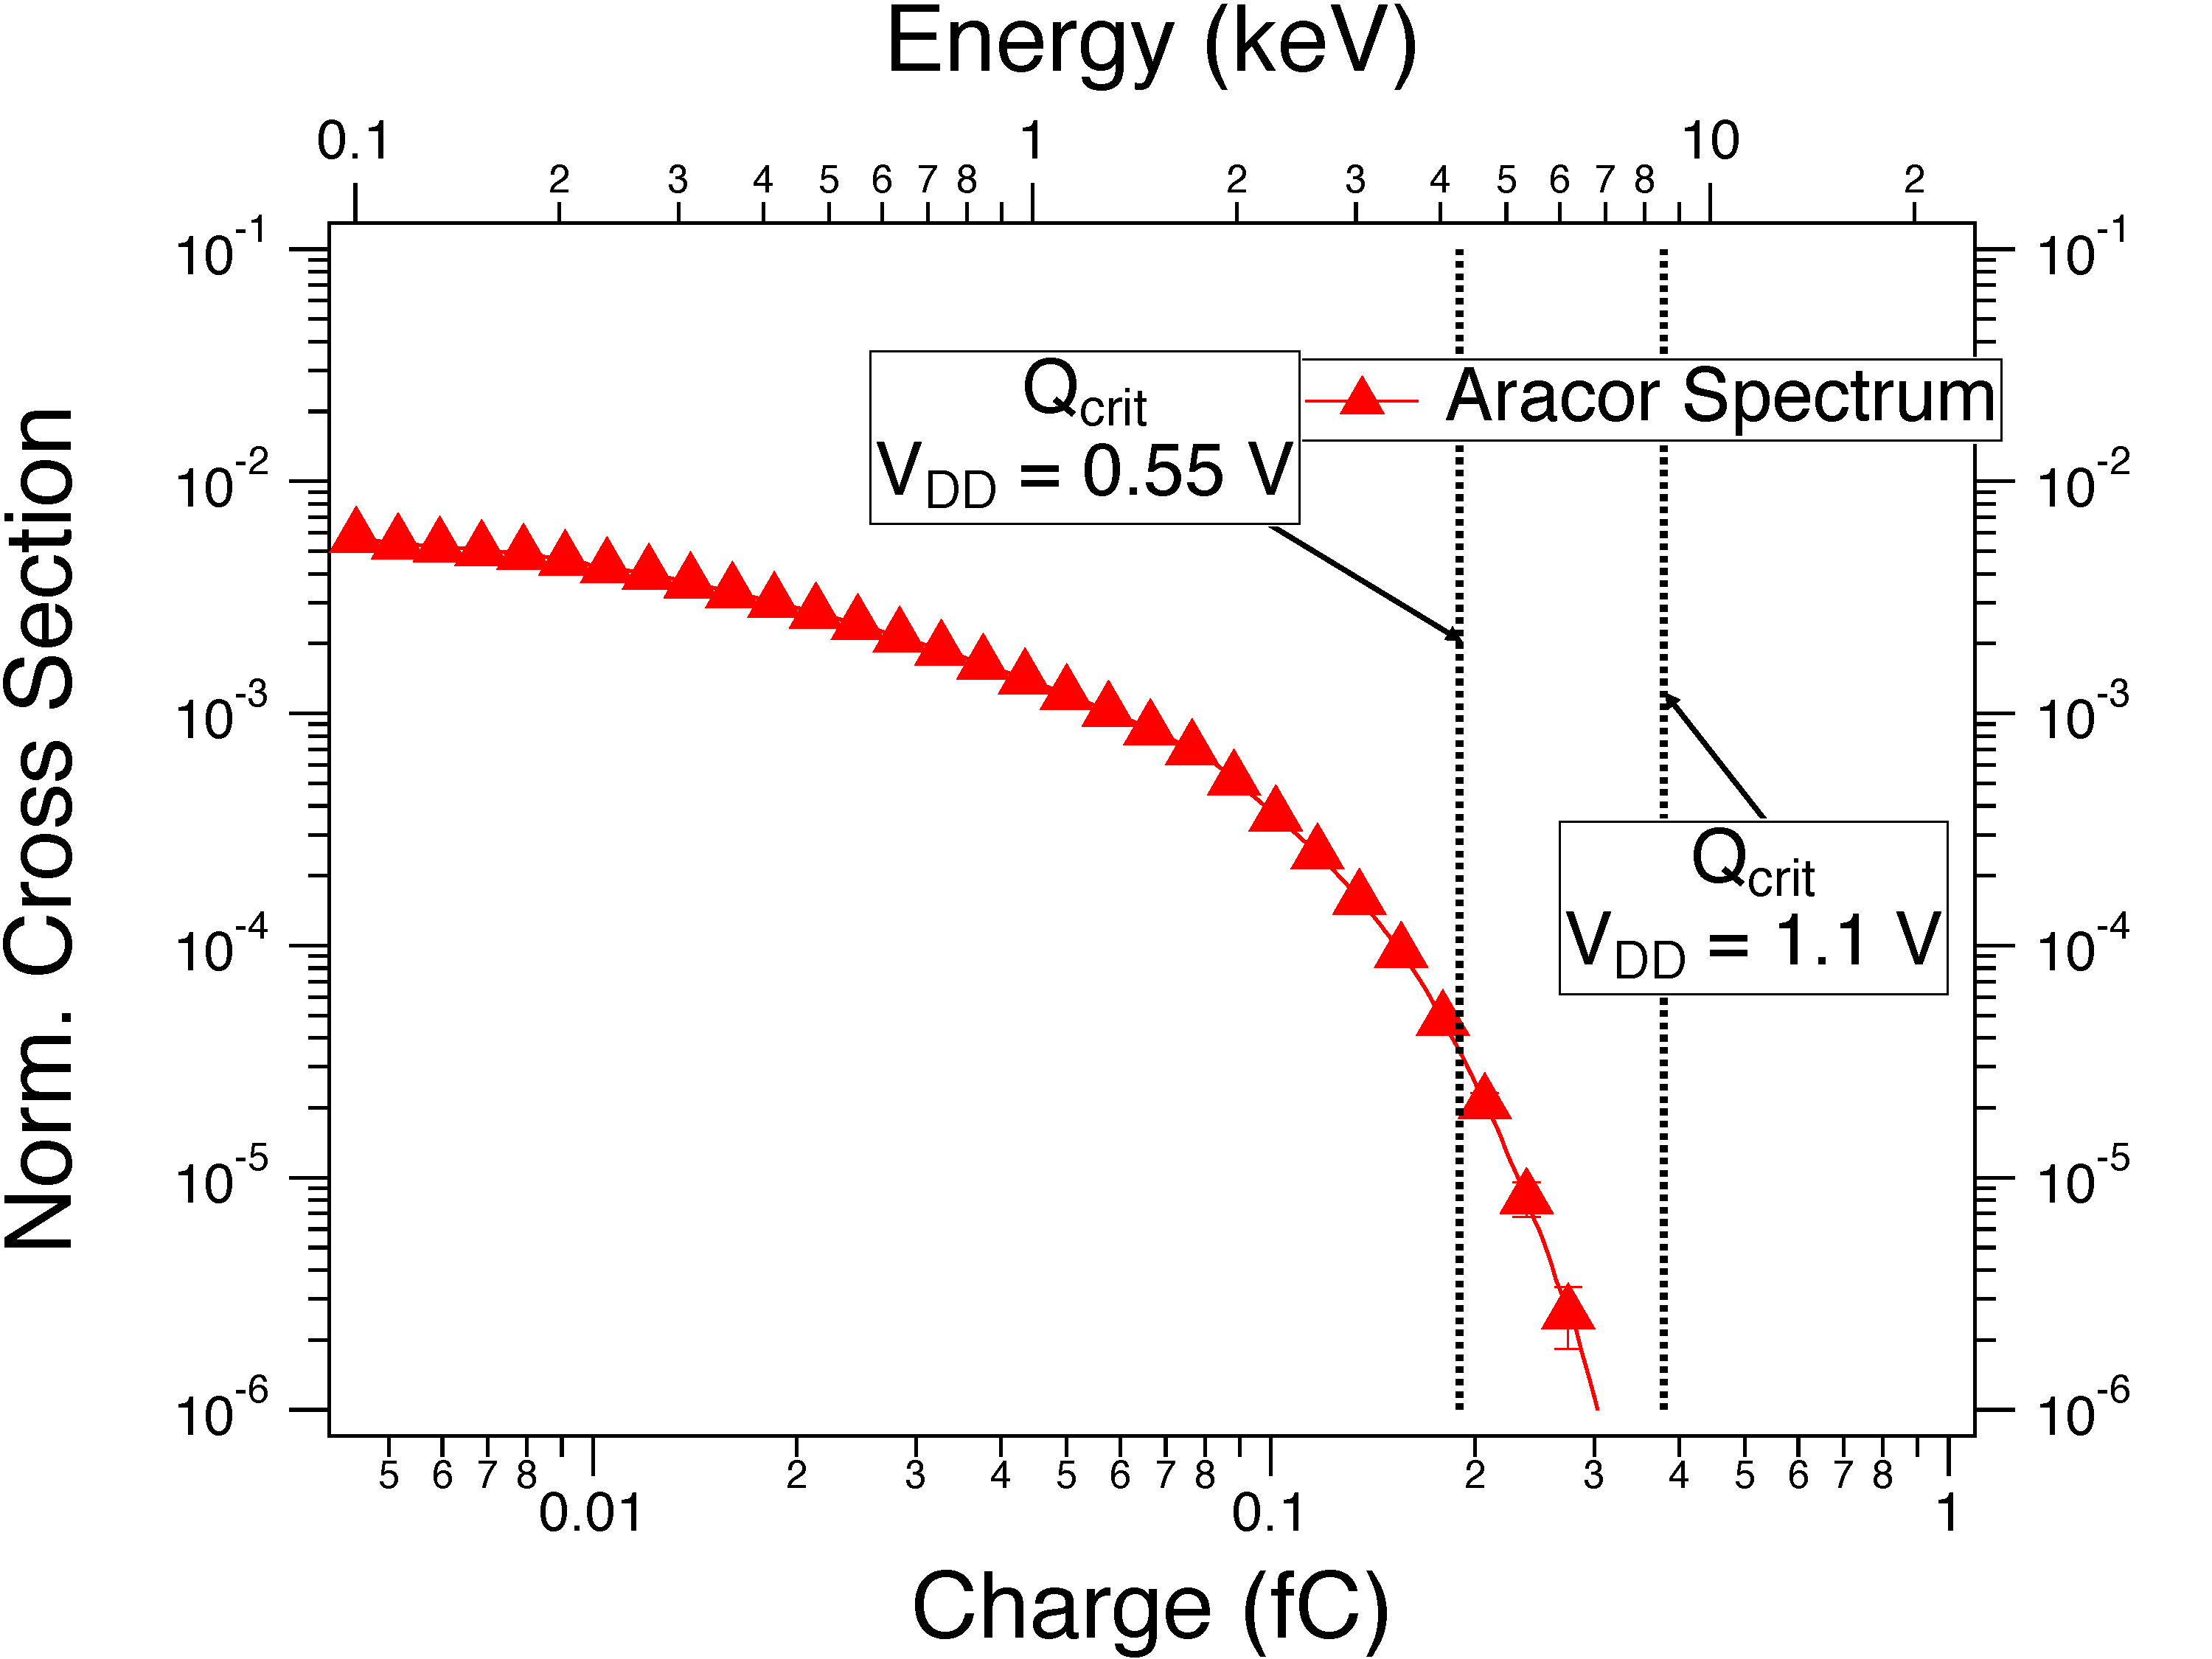
\includegraphics[width=5in]{full_aracor_spectrum_xrays_ppt.pdf}
   \caption{MRED simulation results of the attenuated ARACOR spectrum, seen in Fig.~\ref{fig:aracor_spectrum}, normally incident on a 45~nm bulk SRAM structure. The vertical black lines represent the lower-limit estimates of critical charge for a 45~nm SRAM. The results provide supporting evidence suggesting that energetic electrons generated by incident X-rays are capable of depositing sufficient energy to exceed the estimated upset threshold.}
   \label{fig:50kev_xrays_ppt}
\end{figure}
The vertical black lines in Fig.~\ref{fig:50kev_xrays_ppt} represent estimates of critical charge for 45~nm SRAMs as in \cite{King:2010cu} for supply voltages of 0.55~V and 1.1~V, which correspond to 0.19~fC and 0.38~fC of generated charge, respectively, and are used to indicate the charge generation required to upset cells.

Simulated integral cross-sections are shown in Fig.~\ref{fig:50kev_xrays_ppt}, indicating that secondary electrons generated by incident X-rays are capable of depositing sufficient energy to exceed the critical charge estimate of a 45~nm SRAM. 
The eventual upsets result from collection of thermalized \emph{e-h} pairs generated by the high-energy electrons. 
These results, suggesting energetic electrons are capable of depositing sufficient ionizing energy to exceed the critical charge of 45~nm SRAMs operating under reduced supply voltage, are consistent with previous computational results reported in \cite{King:2010cu, King:2012cb}. 
The normalized cross-section in Fig.~\ref{fig:50kev_xrays_ppt} at a supply voltage of 0.55~V agrees with experimental test results from Test Chip D in Fig.~\ref{fig:xray_exp_seus} within a factor of two. 
These results suggest that the 45~nm SRAM is relatively insensitive to single-electron SEU at nominal supply voltage, consistent with the SEU data in Fig.~\ref{fig:xray_exp_seus}. 

Further analysis of individual events shows that single electrons scattering within the sensitive volumes representative of sub-65~nm bulk and SOI technology frequently deposit energy in excess of the estimated critical charge thresholds in Fig.~\ref{fig:50kev_xrays_ppt}.
Fig.~\ref{fig:50nm_cube_silicon} shows 10~keV electrons transporting through a 500~nm silicon cube and depositing 2.1~keV and 2.6~keV within an embedded 50~nm cube as shown in Figs.~\ref{fig:50nm_cube_2.1_keV} and \ref{fig:50nm_cube_2.6_keV}, respectively. 
Each event shown in Fig.~\ref{fig:50nm_cube_silicon} results in the generation of additional nearly free electrons, in either a single or multiple scattering events, that subsequently transport entirely within the sensitive volume structure, losing all of their energy and reabsorbing into the material.
While the incident electron does not stop within the 50~nm silicon cube in either of the events depicted in Fig.~\ref{fig:50nm_cube_silicon}, energy is transferred to secondary electrons.
The total energy deposited in these volumes exceeds the estimation of critical energy required to produce a SEU in the sub-65nm~nm bulk and SOI technology operated at reduced voltage \cite{Rodbell:2007vl}.
\begin{figure}[htbp]
        \centering
        \subfigure[]{
            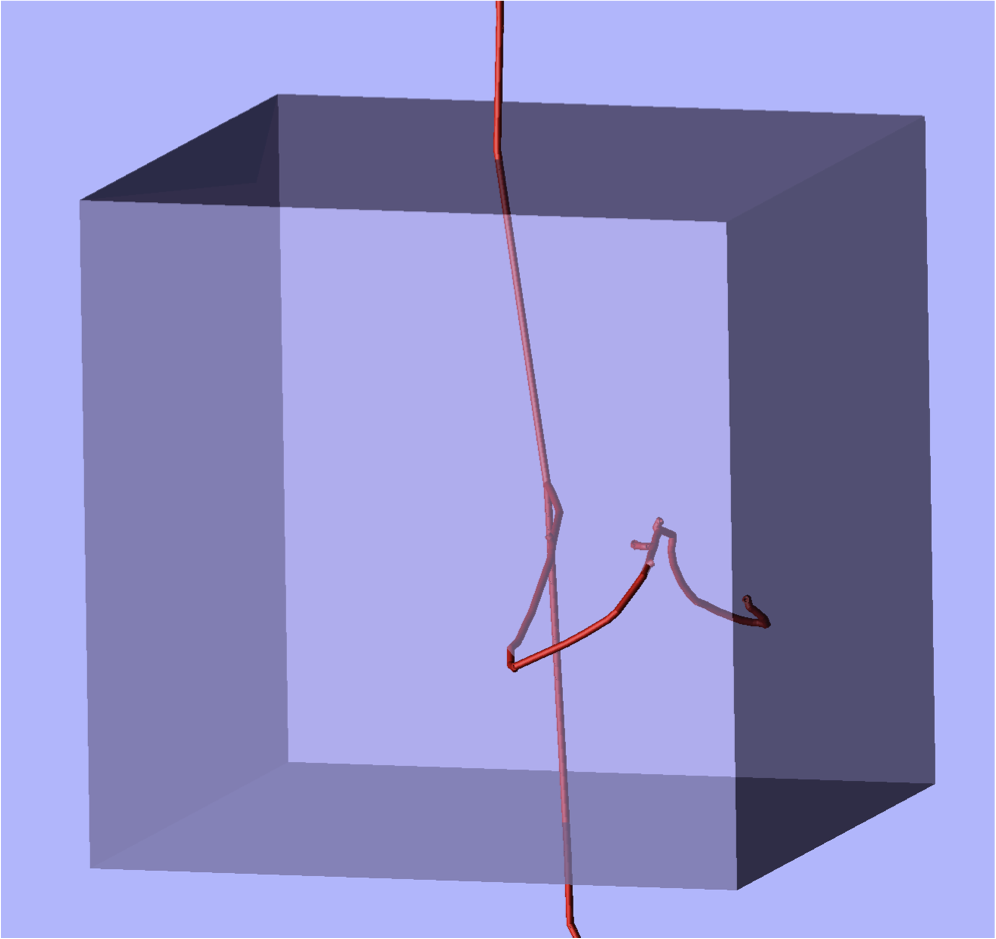
\includegraphics[width=3.25in]{50-nm-cube-10kev-electron-2pt1kev.png}%
            \label{fig:50nm_cube_2.1_keV}
        }
        \subfigure[]{
            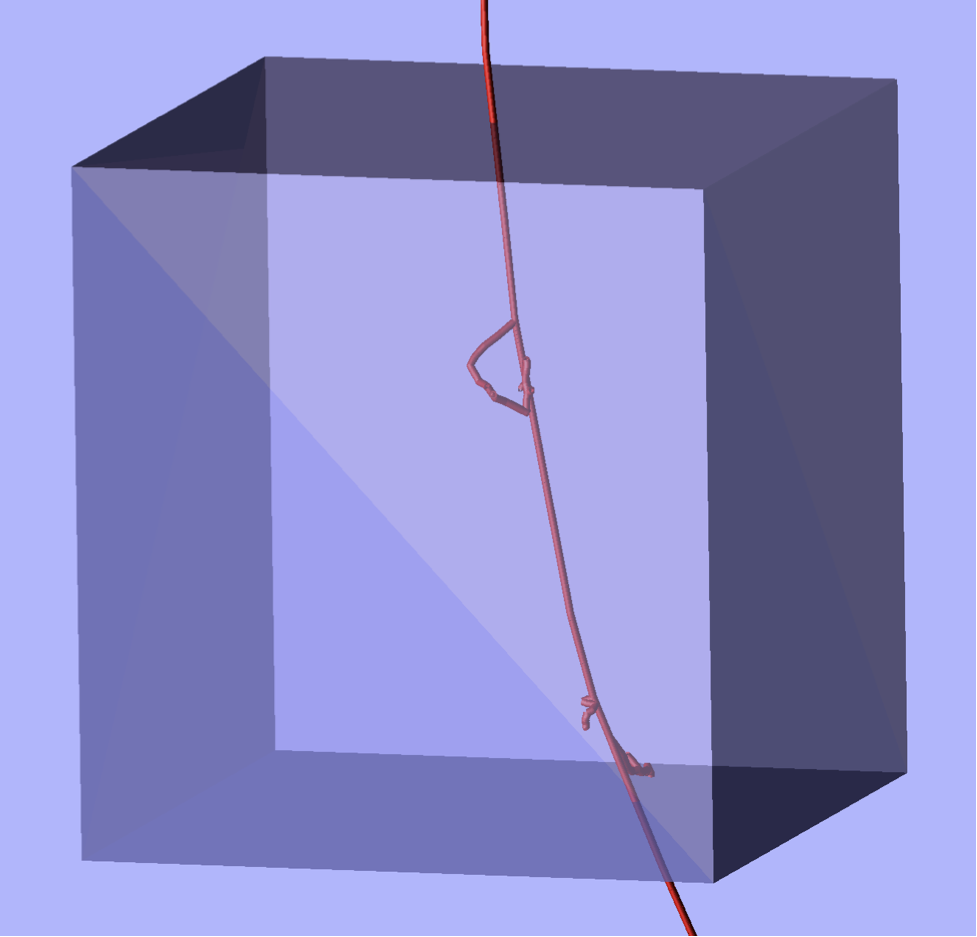
\includegraphics[width=3.25in]{50-nm-cube-10kev-electron-2pt6kev.png}%
            \label{fig:50nm_cube_2.6_keV}
        }
        \caption{Incident 10~keV electrons/$\delta$-rays are shown scattering in a 50~nm cube of silicon. Event \ref{fig:50nm_cube_2.1_keV} shows a 2.1 keV energy deposition event that produces additional electrons/$\delta$-rays in a chain of inelastic scattering events. Event \ref{fig:50nm_cube_2.6_keV} shows a 2.6 keV energy deposition event that produces several tertiary electrons/$\delta$-rays in a series of inelastic scattering events.}
        \label{fig:50nm_cube_silicon}
\end{figure}

% Deeper inspection shows that there is significant difficulty in accurately calibrating the sensitive volume model and estimating critical charge for sub-45~nm SRAMs under reduced bias conditions.
A comparison of simulation and experimental cross-sections, normalized to SRAM cell area, is shown in Fig.~\ref{fig:sim-vs-exp-norm-cross-section}, which shows reasonable agreement between the simulation and experimental results for the 45~nm bulk SRAM.
This comparison shows that MRED agrees with experimental results within a factor of 2--5 for an applied bias between 0.5~V and 0.7~V.
Simulation results underestimate the normalized upset cross-section for applied bias conditions less than 0.55~V and are conservative for higher bias conditions.
The SEU bias dependence of simulation results differs slightly from the experimental results, exhibiting a smaller slope as a function of applied bias than is shown in experimental work. 
To date, the bias dependence of sensitive volume geometries has not been investigated for SRAMs frabricated in advanced technology nodes.

\begin{figure}[tb]
    \begin{center}
        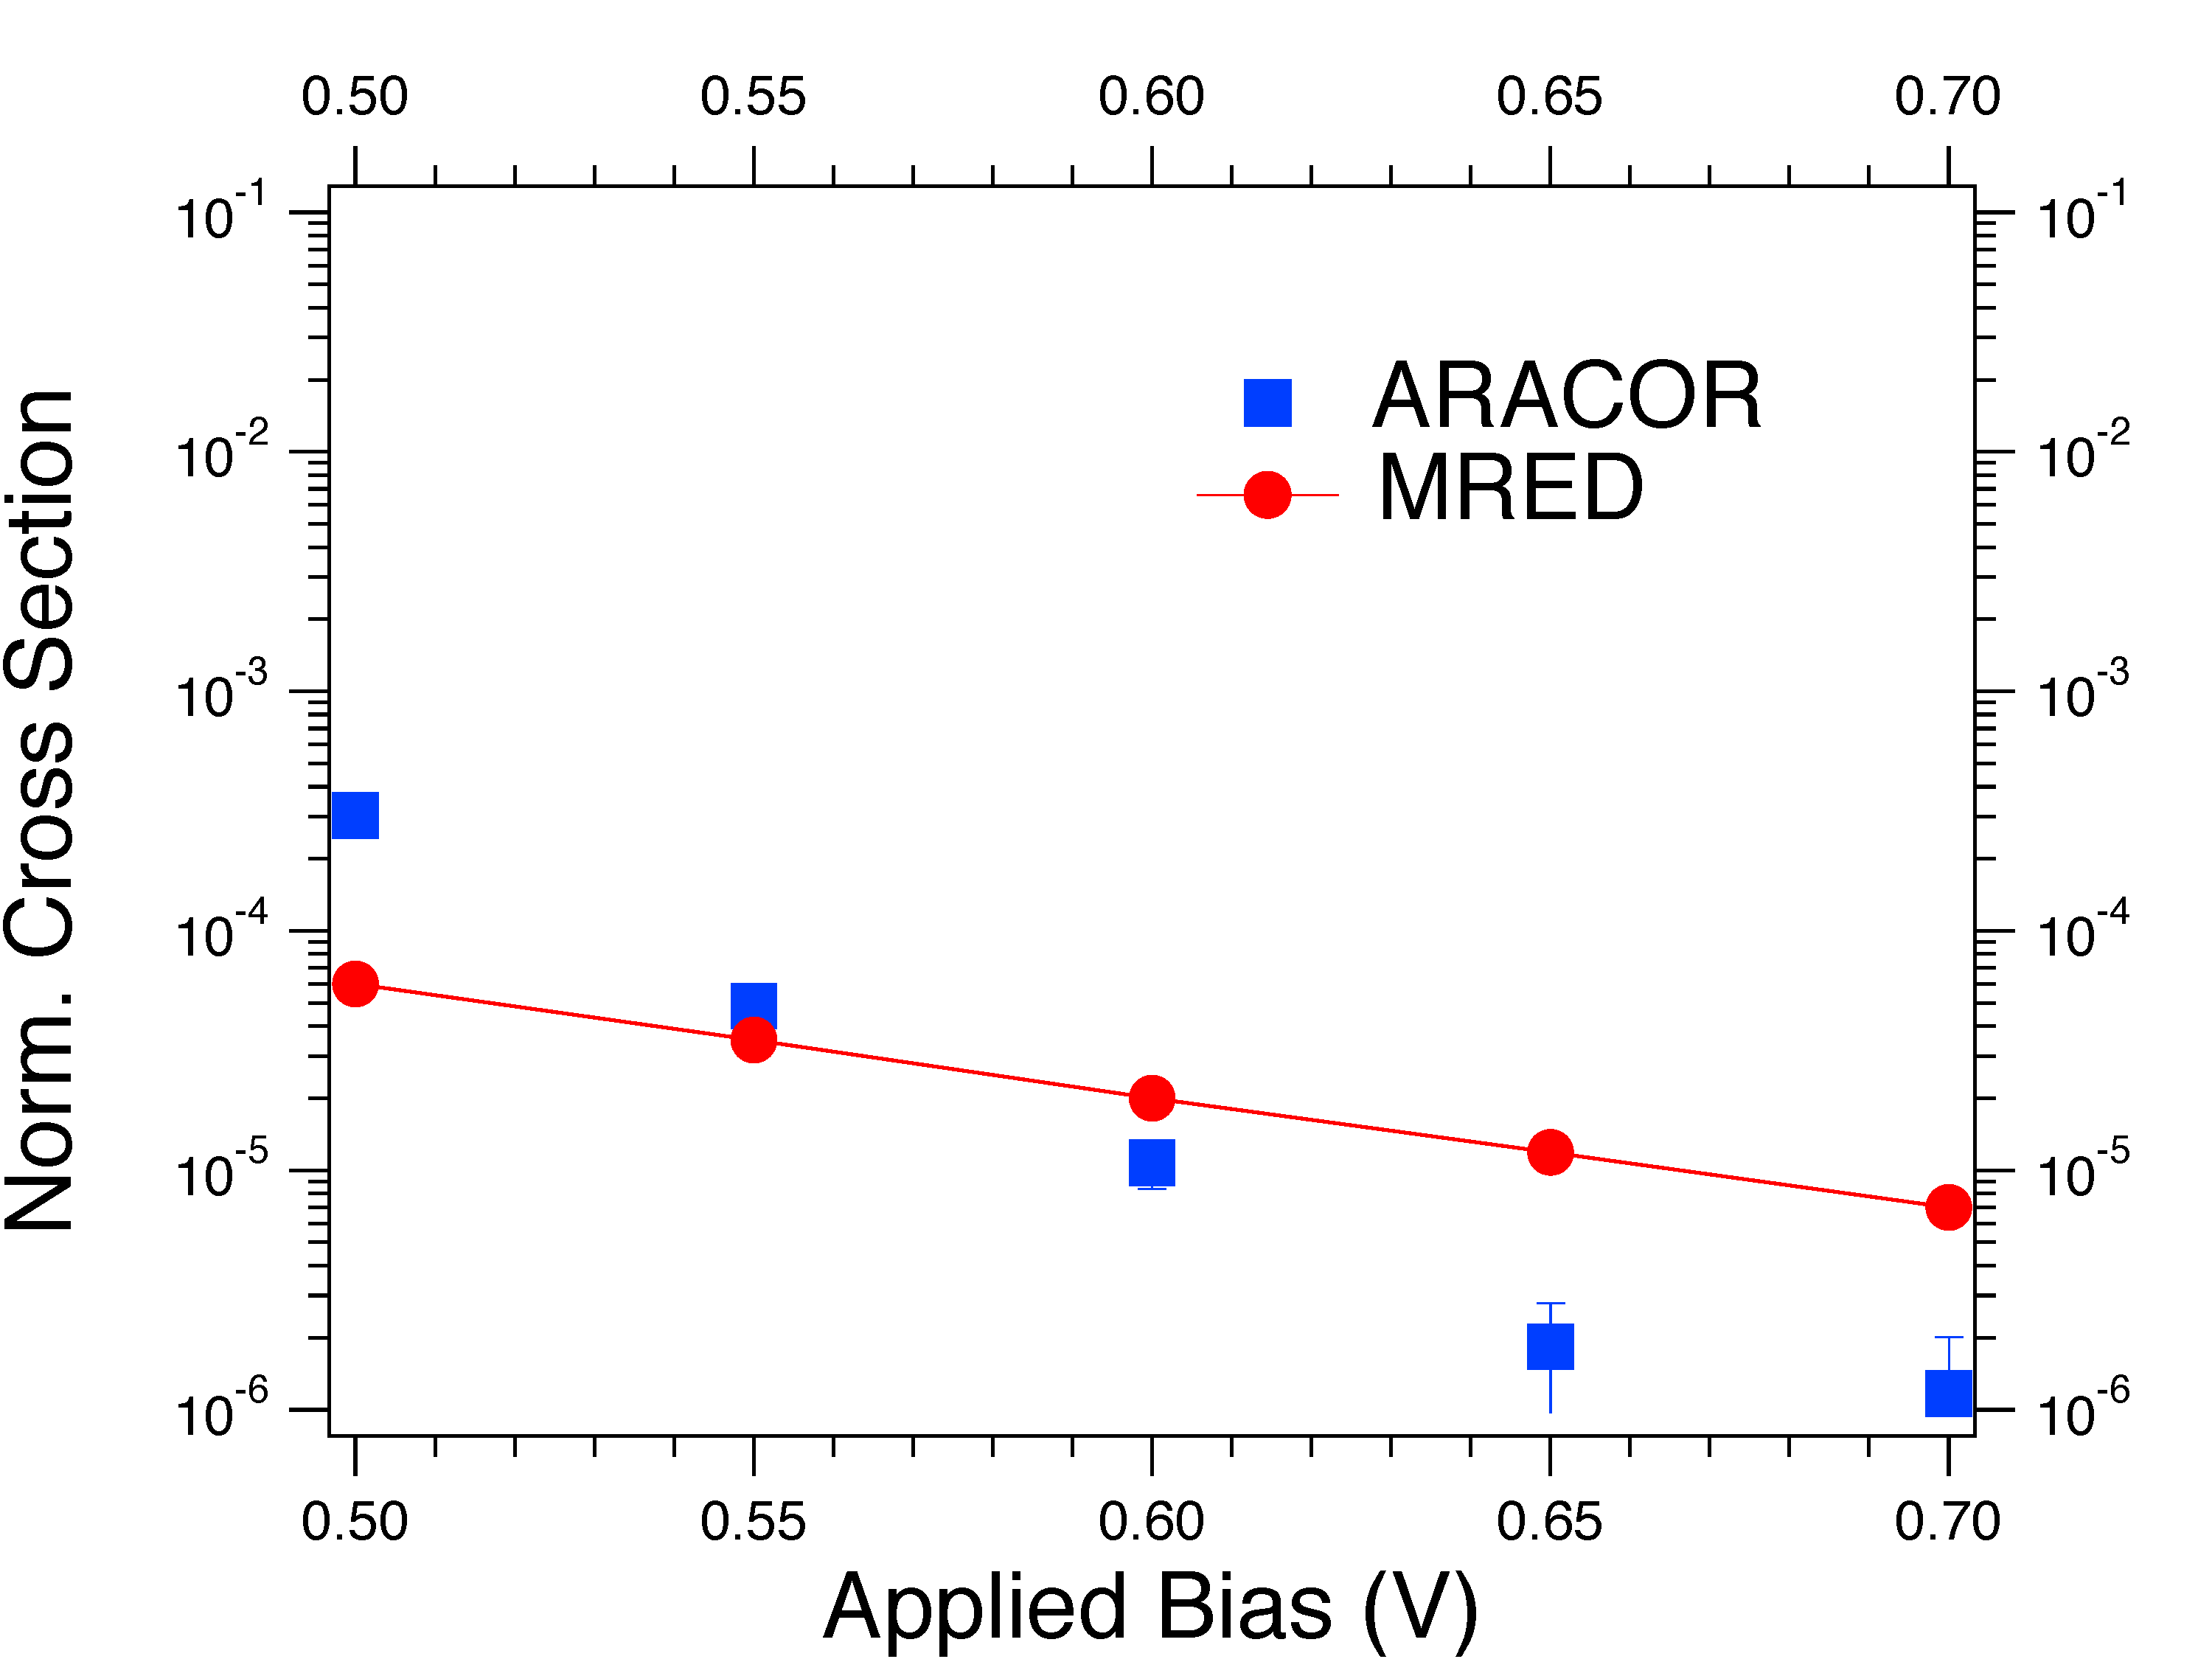
\includegraphics[width=5in]{sim-vs-exp-norm-cross-section.pdf}
    \end{center}
    \caption{Comparison of simulated versus experimental normalized cross-section for Test Chip D, a 45~nm bulk SRAM.}
    \label{fig:sim-vs-exp-norm-cross-section}
\end{figure}

The sensitive volume geometry chosen in this research was a static, uncalibrated model for the simulation results reported in Figs.~\ref{fig:50kev_xrays_ppt} and \ref{fig:sim-vs-exp-norm-cross-section}.
Given that the sensitivity of the SRAM cell is expected to increase under reduced bias conditions the dimensions of the simulated sensitive volume are a potential source of error in the above simulation results.
Additionally, a \emph{simple} model (see Equation~\ref{eq:qcrit}) was used to estimate the critical charge of the 45~nm SRAM due to the lack of models and process details necessary to extract critical charge information using BSIM/SPICE for the 45~nm technology node.
Increased fidelity in approximating the critical charge can yield significant differences in the extrapolated critical charge values shown in Fig.~\ref{fig:sim-vs-exp-norm-cross-section}.
It is clear from these results that a static collection volume, one that is invariant with respect to supply voltage, cannot accurately reproduce the complete bias-dependent cross-section response of SRAMs that are sensitive to electron-induced SEUs.
Without extensive effort, readily available SEU data, and process details, it is difficult to simultaneously calibrate a bias dependent sensitive volume geometry, charge collection model, and critical charge parameters to achieve an exhaustive model of SRAMs in any technology node.
Despite the simple approximations and geometrical assumptions, Fig.~\ref{fig:sim-vs-exp-norm-cross-section} shows very good agreement with experimental results over a range of bias conditions where the fidelity of those estimations is reasonable.
Trends showing decreased sensitivity of 45~nm SRAMs at higher supply voltage conditions is observed in simulation data and the normalized cross-section results are comparable with that of the experimental results.

These simulation results confirm that energy deposition from energetic electrons generated in photoabsorption events is the most likely explanation for the experimentally observed upsets in Fig.~\ref{fig:xray_exp_seus}. %
% section simulation_of_x_ray_energy_deposition_in_srams (end)

\section{Electron-Induced SEU Event Rates} % (fold)
\label{sec:electron_induced_seu_event_rates}
Comparing the experimental cross-sections in Figs.~\ref{fig:28nm_xray_muon_proton} and \ref{fig:45nm_xray_muon_proton} indicates the sensitivity of SRAMs to protons, muons, and electron, however, event rates depend on the flux of these particles for different environments. 
Trapped electrons form two different belts in the near Earth radiation environment, each with distinct characteristics \cite{Bourdarie:kj, Xapsos:2013cu}.
The Jovian electron environment is equally formidable as it contains electrons with higher energy and flux than that of the near-Earth environment.
This section investigates the potential for electron-induced SEUs in the near-Earth and Jovian environments using MRED simulations.

\begin{figure}[htbp]
    \begin{center}
        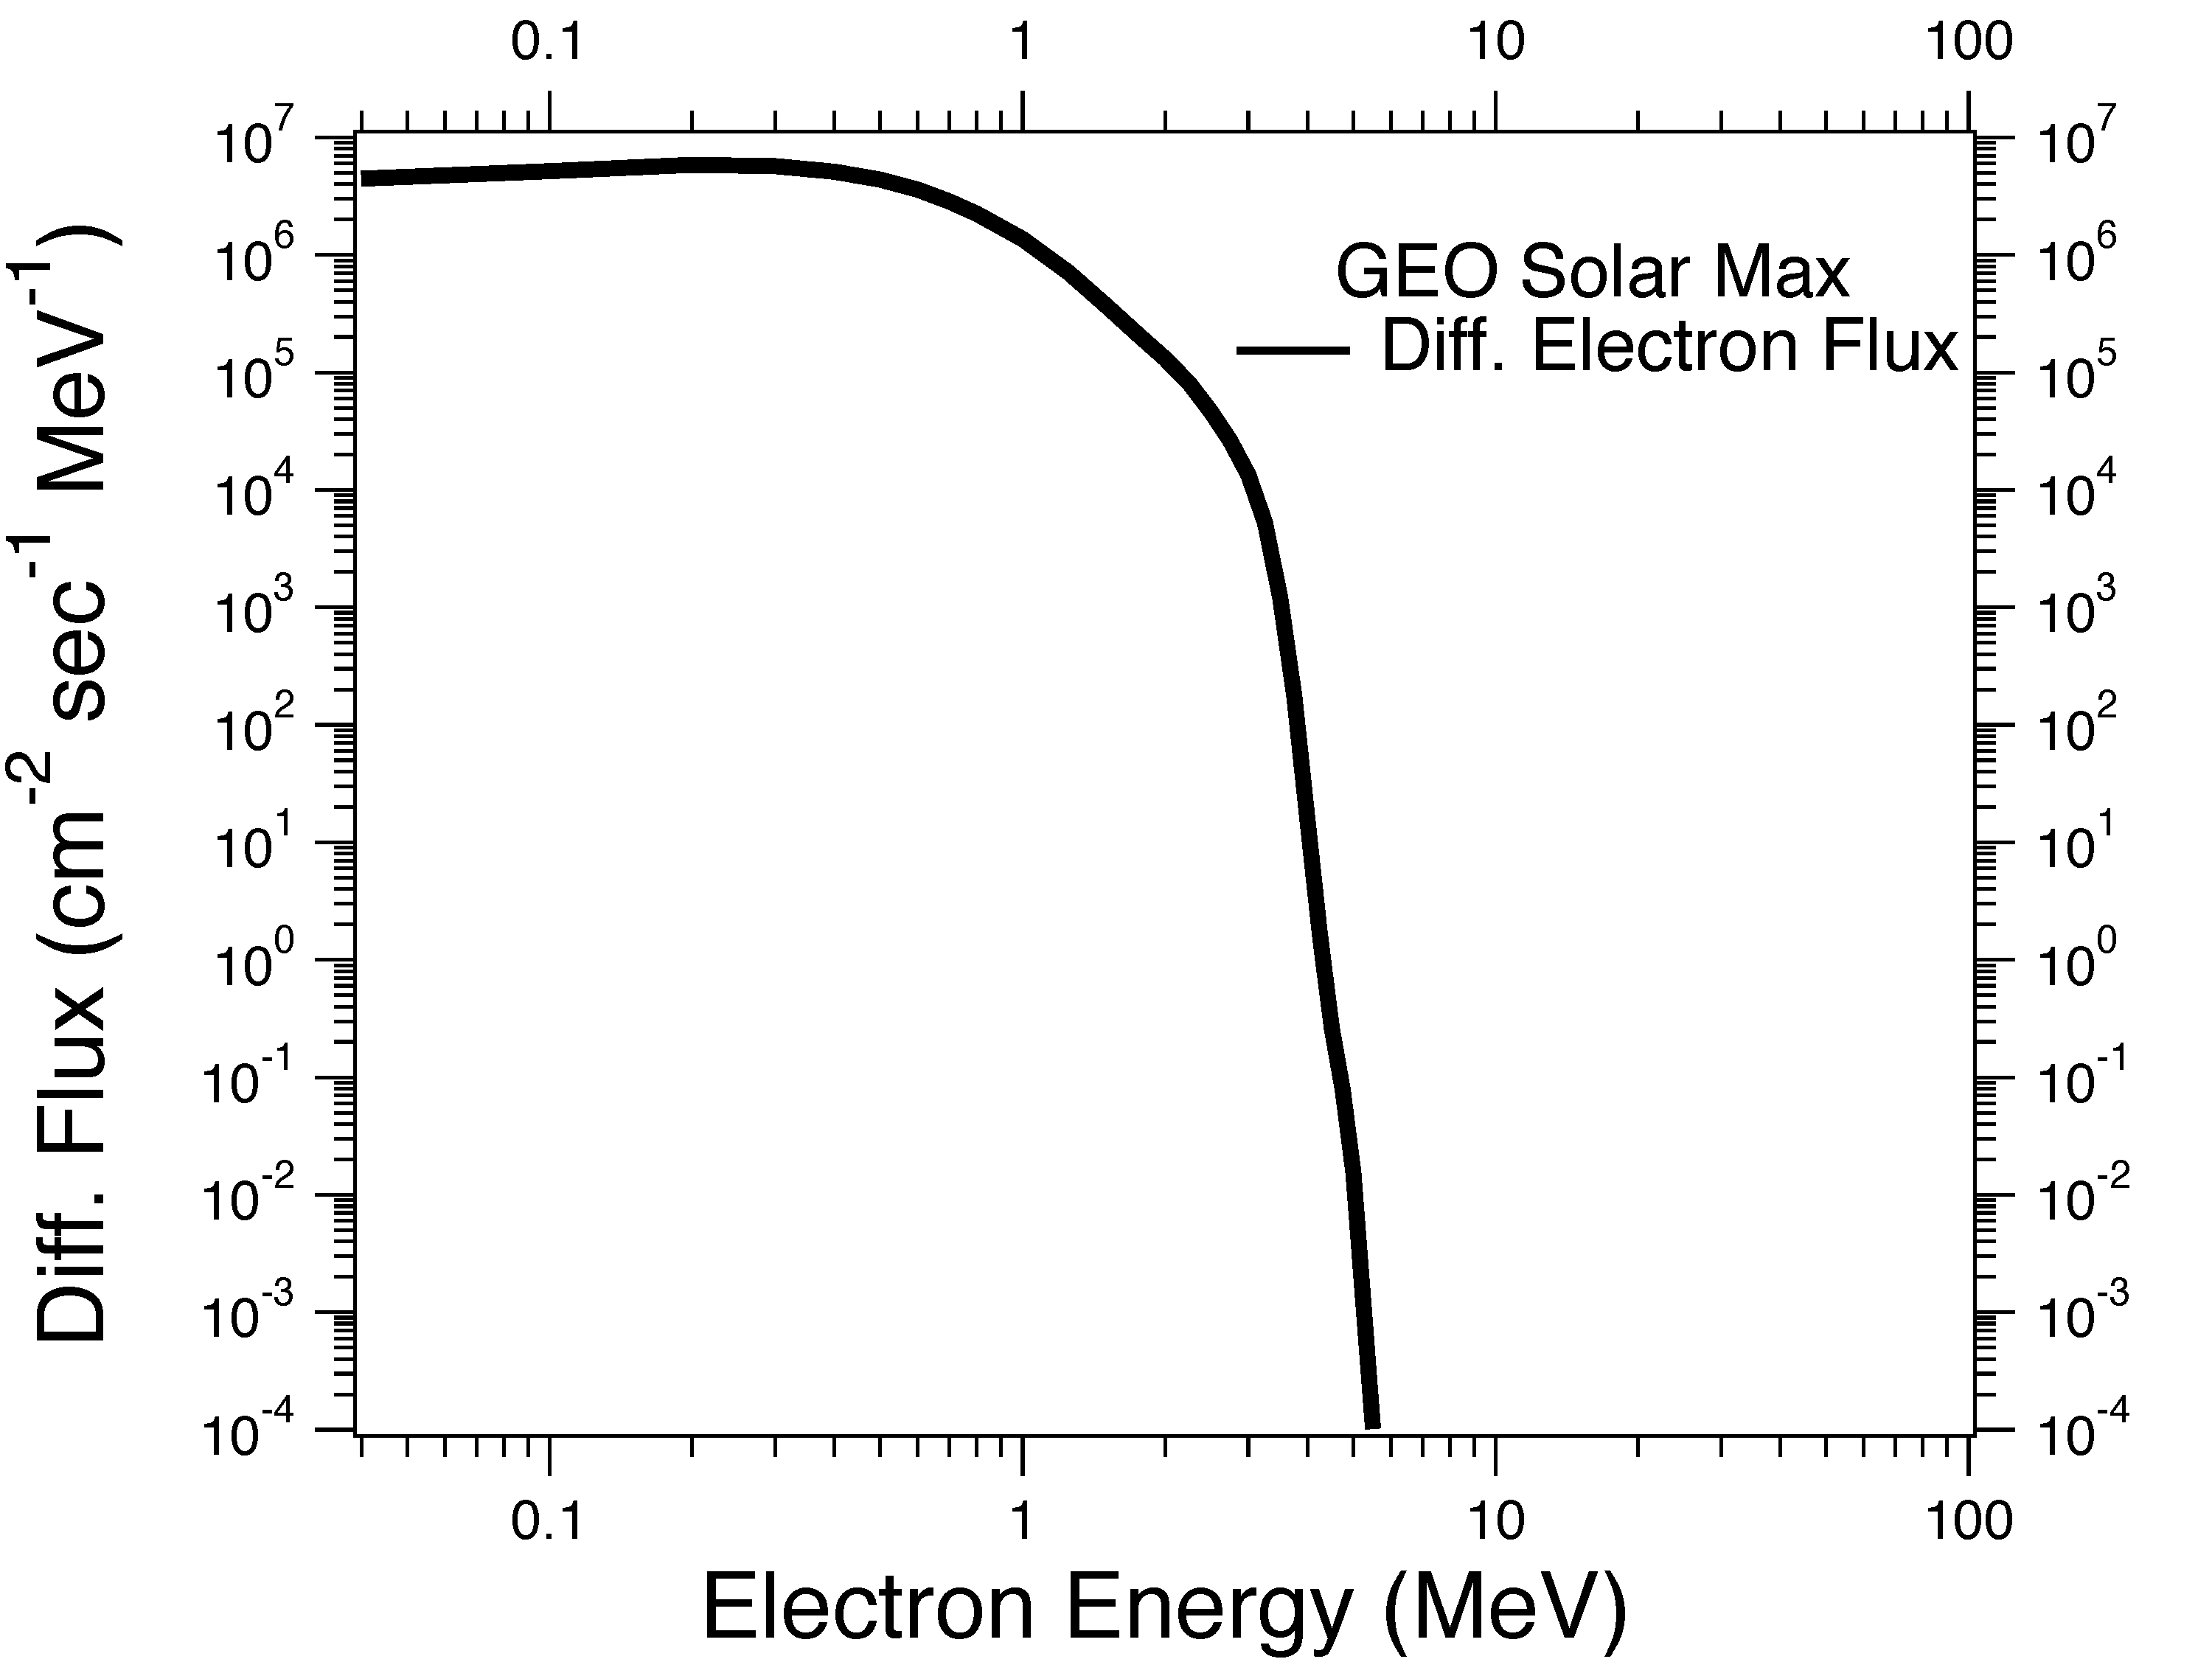
\includegraphics[width=6in]{geo_max_rate_pred_ae8_spec_ppt.pdf}
    \end{center}
    \caption{The differential flux spectrum of incident electrons is plotted using the AE-8 description of the electron environment, at geosynchronous orbit during solar maximum with 150~mils aluminum shielding. It is noted that 150~mils of aluminum is sufficient to shield the simulated SRAM from protons in this environment.}
    \label{fig:ae8_spec_ppt}
\end{figure}

Simulations were performed to estimate SEU event rates for trapped electrons at geosynchronous orbit during solar maximum with 150~mils of aluminum shielding using spectra obtained from the AE-8 model for the near-Earth environment.
The differential flux spectrum of incident electrons through 150~mils of aluminum shielding is plotted in Fig.~\ref{fig:ae8_spec_ppt}.
% The presence of 150~mils of aluminum shielding was sufficient to stop the entire spectrum of protons under the same conditions.
The trapped electron environment described in Fig.~\ref{fig:ae8_spec_ppt} is much more energetic than the generated electron spectrum used in X-ray experiments described in Chapter~\ref{cha:experimental_investigation_of_electron_induced_seus}.
The most energetic electrons at geosynchronous orbit during solar maximum have energy of approximately 10~MeV, which would require more than 500~mils of aluminum shielding to attenuate completely \cite{Bourdarie:kj,Xapsos:2013cu}.

Characteristics of the Jovian electron environment were discussed in Section~\ref{sub:trapped_particle_environment}.
Simulations of electron-induced SEU event rates were performed for the differential flux spectrum shown in Fig.~\ref{fig:jovian-int-flux-spectrum}.
Additionally, attenuated differential electron and proton spectra are presented in Figs.~\ref{fig:jov-eur-elec-flux-env} and \ref{fig:eur-prot-flux-env} showing the impact of 100~mils, 730~mils, and 870~mils of aluminum shielding on the differential flux of electrons and protons during the Jovian and Europa phases of the Juno spacecraft mission to the Jupiter planetary system.
The electron flux spectrum shown in Fig.~\ref{fig:jov-eur-elec-flux-env} indicates that 100~mils of aluminum shielding has minimal impact on the flux of low-energy electrons ($<$100~keV).
The proposed higher shielding thicknesses of 730 and 870~mils, however, have a significant impact on the flux of low-energy electrons, reducing it by over two orders of magnitude.

\begin{figure}[htbp]
    \begin{center}
        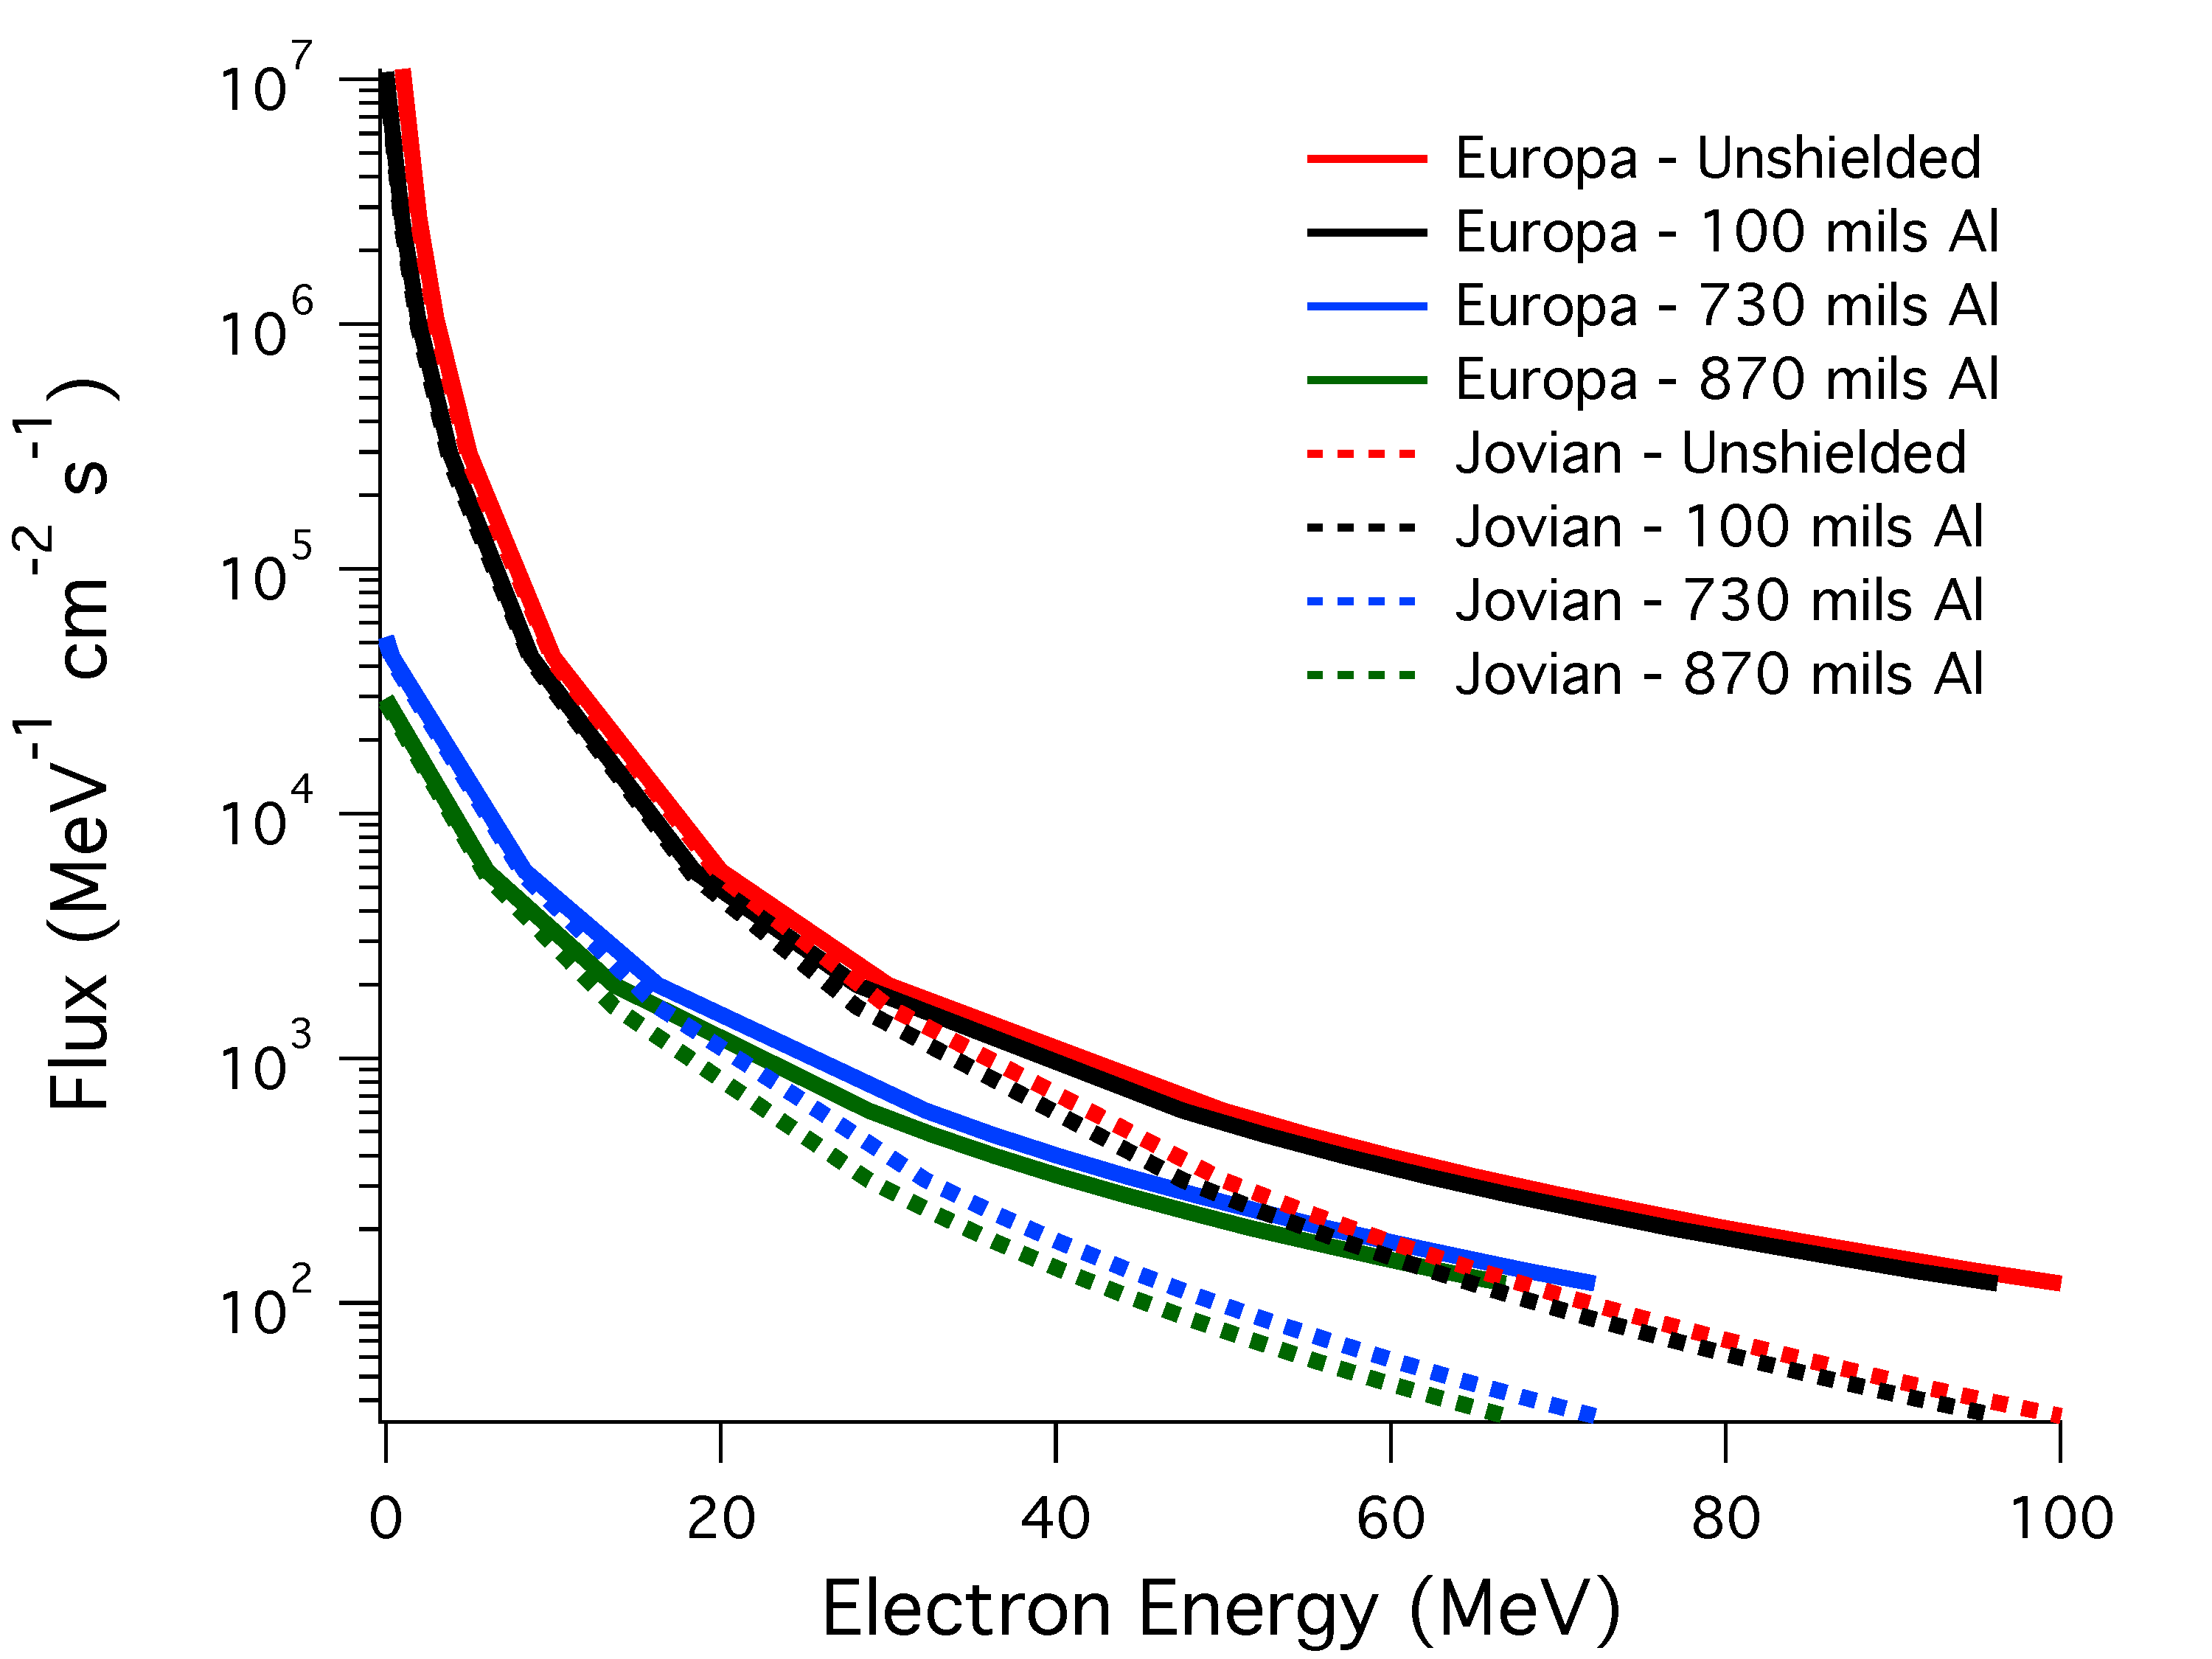
\includegraphics[width=6in]{jov-eur-elec-flux-env.pdf}
    \end{center}
    \caption{Differential electron flux for unshielded, 100~mils, 730~mils, and 870~mils of aluminum shielding in the Jovian and Europa tour phase of the Juno spacecraft mission to the Jupiter planetary system.}
    \label{fig:jov-eur-elec-flux-env}
\end{figure}

\begin{figure}[htbp]
    \begin{center}
        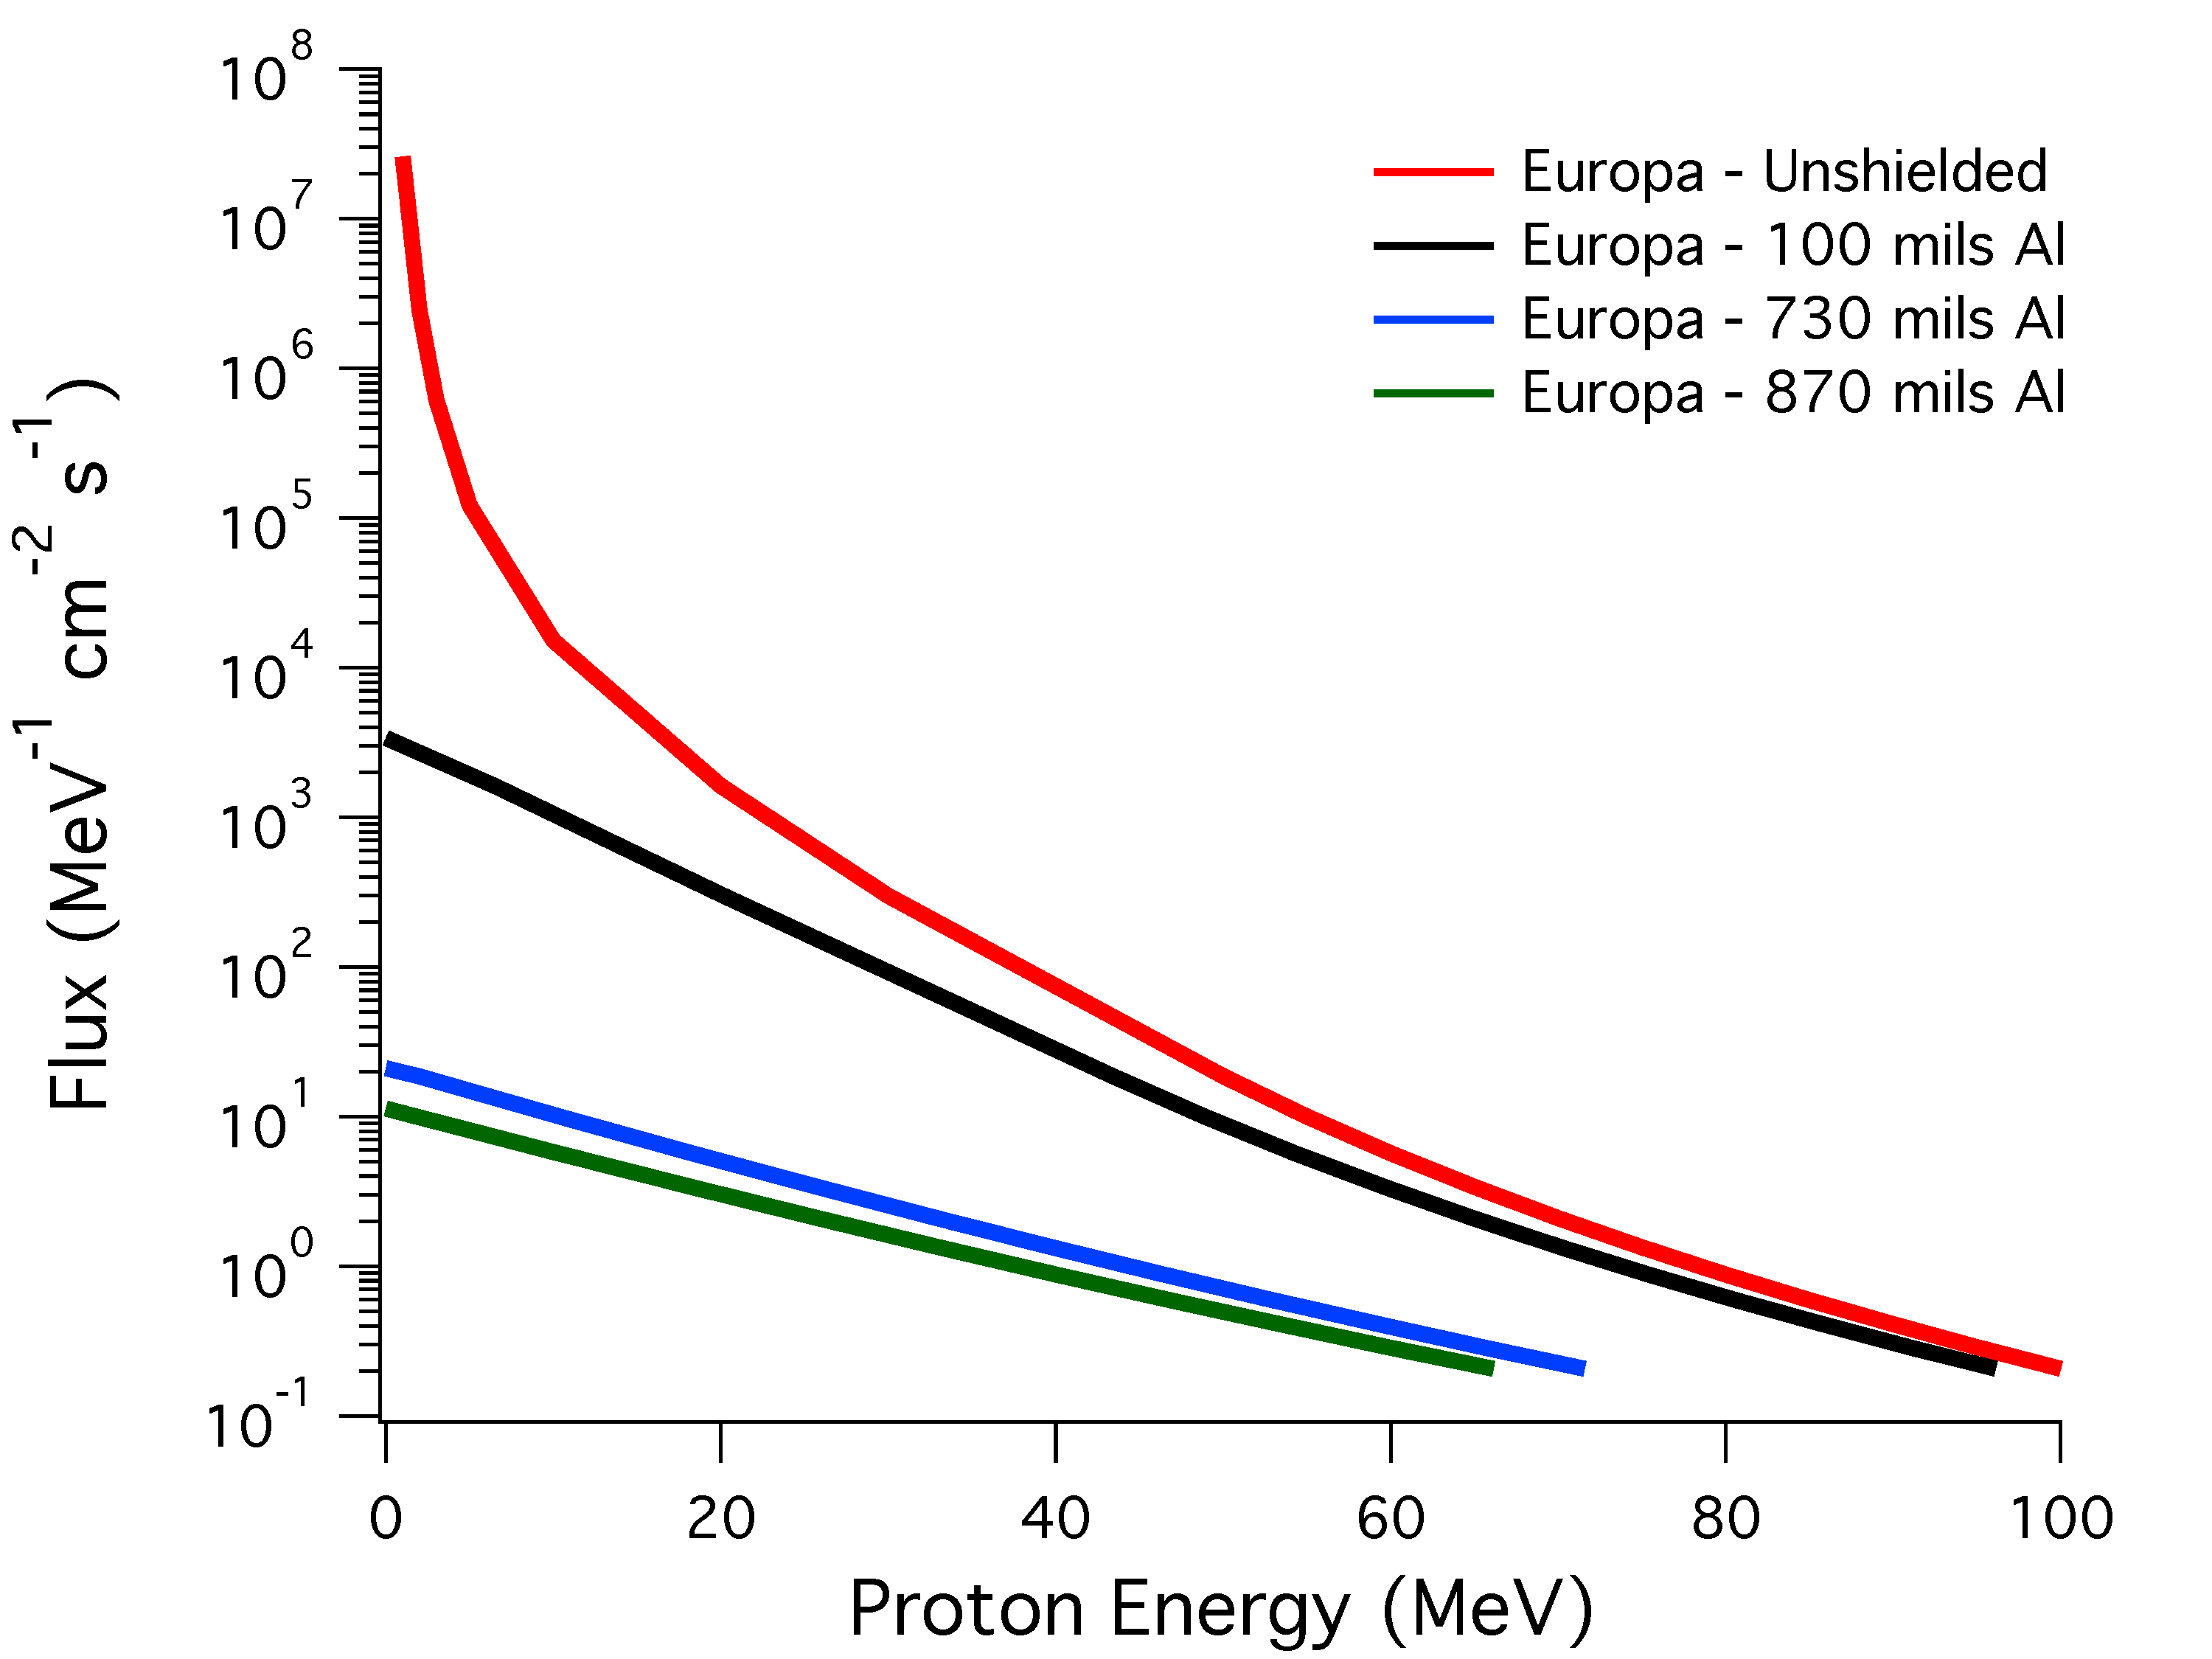
\includegraphics[width=6in]{eur-prot-flux-env.pdf}
    \end{center}
    \caption{Differential proton flux for unshielded, 100~mils, 730~mils, and 870~mils of aluminum shielding in the Europa tour phase of the Juno spacecraft mission to the Jupiter planetary system.}
    \label{fig:eur-prot-flux-env}
\end{figure}

In contrast to electrons, Fig.~\ref{fig:eur-prot-flux-env} shows that shielding of protons has a much greater impact on the proton flux in the Europa environment, effectively reducing the high-flux region of low-energy ($<$5~MeV) protons from the unshielded spectrum.
As mentioned previously, the flux and energy of electrons and protons in the Jovian environment is significantly higher than that of the near-Earth environment.
The simulations of the Jovian environment investigate an unshielded part, and parts with varying shielding thicknesses, in the Europa and Jovian tour segments of the Juno spacecraft mission.
% Since the simulated part is unshielded, these simulations represent a ``worst-case'' response since the device sees the full spectrum of a high flux environment.

\begin{figure}[htbp]
    \begin{center}
        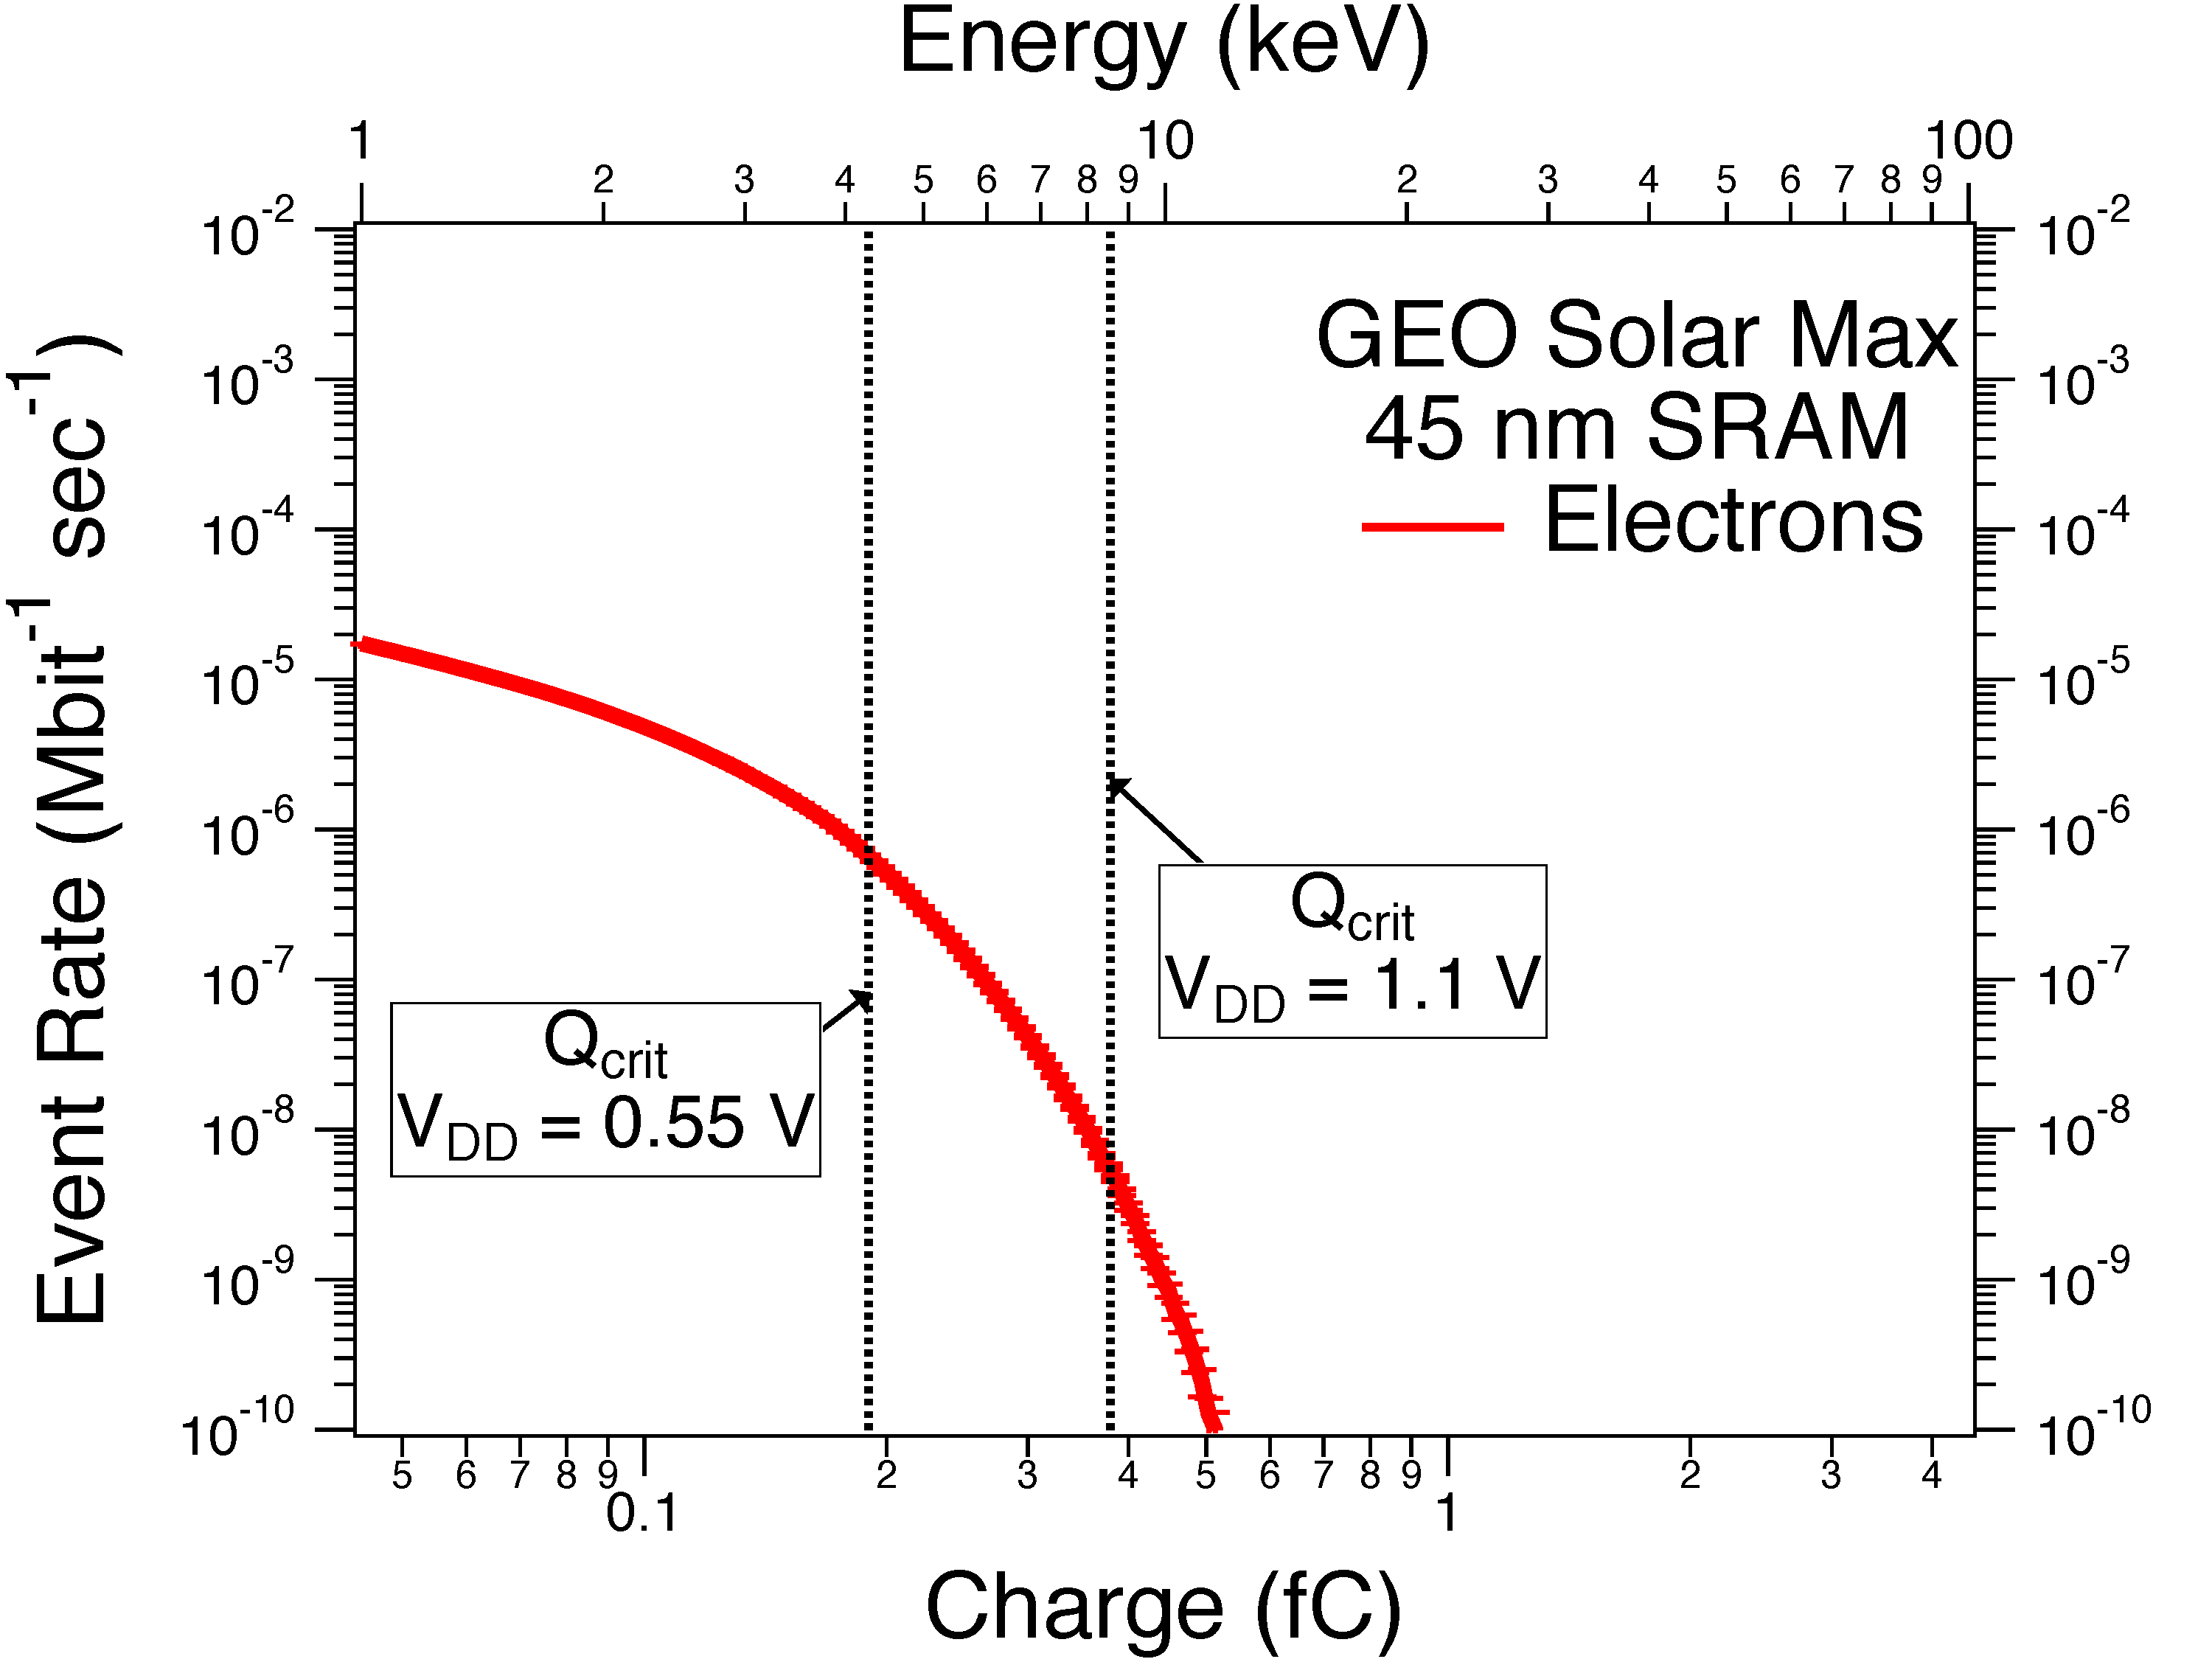
\includegraphics[width=6in]{geo_max_rate_pred_ae8_ppt.pdf}
    \end{center}
    \caption{MRED simulations performed on the 45~nm structure from Fig.~\ref{fig:50kev_xrays_ppt} using the AE-8 description of the electron environment, at geosynchronous orbit during solar maximum with 150~mils aluminum shielding. Simulation results show that the event rate of electrons is small for devices operated under nominal supply voltage, as seen in \ref{fig:geo_max_rate_pred_ae8_ppt}. However, more sensitive devices will experience a significant increase in single electron events. These results suggest that operating SRAMs under reduced bias conditions will result in a dramatic increase in single electron events.}
    \label{fig:geo_max_rate_pred_ae8_ppt}
\end{figure}

MRED was used to model the interaction of the particle spectrum with the semiconductor materials. 
The material structure is identical to the structure from Fig.~\ref{fig:50kev_xrays_ppt}, corresponding to a 45~nm bulk SRAM.
Fig.~\ref{fig:geo_max_rate_pred_ae8_ppt} shows the resulting simulated event rates (left/right axis) as a function of generated charge (bottom axis) or energy deposited (top axis) within the sensitive volume of a single 45~nm SRAM cell for the near-Earth environment. 
Electron energy deposition events rarely exceed 10~keV, which is consistent with Fig.~\ref{fig:50kev_xrays_ppt} and previous studies of $\delta$-rays \cite{King:2010cu, King:2012cb}. 
Fig.~\ref{fig:geo_max_rate_pred_ae8_ppt} demonstrates the rare nature of electron-induced SEU events in the near-Earth space radiation environment, indicating that many years of flight time may elapse before the observation of such an event is expected for a typical 45~nm bulk SRAM operating under nominal bias conditions.  

Fig.~\ref{fig:geo_max_rate_pred_ae8_ppt} shows that the electron-induced SEU event rates depends strongly on the critical charge of the SRAM; a reduction of critical charge from 0.4~fC to 0.2~fC results in a change in event rate of approximately two orders of magnitude. 
Employing more sensitive SRAM technologies or operating at reduced supply voltage conditions has a direct and significant impact on SRAM error rates. 
In contrast, total error rate predictions for a 65~nm SRAM at geosynchronous orbit in the solar minimum environment are on the order of 2.4$\times$10$^{-6}$~Mbit$^{-1}$~sec$^{-1}$ \cite{Sierawski:2009ka}.
At geosynchronous orbit in ``worst-day'' conditions, error rates for the same 65~nm SRAM are as high as 3.6$\times$10$^{-3}$~Mbit$^{-1}$~sec$^{-1}$ \cite{Sierawski:2009ka}.
This indicates that the error rates at geosynchronous orbit of larger technology nodes with higher critical charge are roughly 2.5--5 orders of magnitude higher than estimates of electron-induced error rates at nominal bias conditions.

\begin{figure}[htbp]
    \begin{center}
        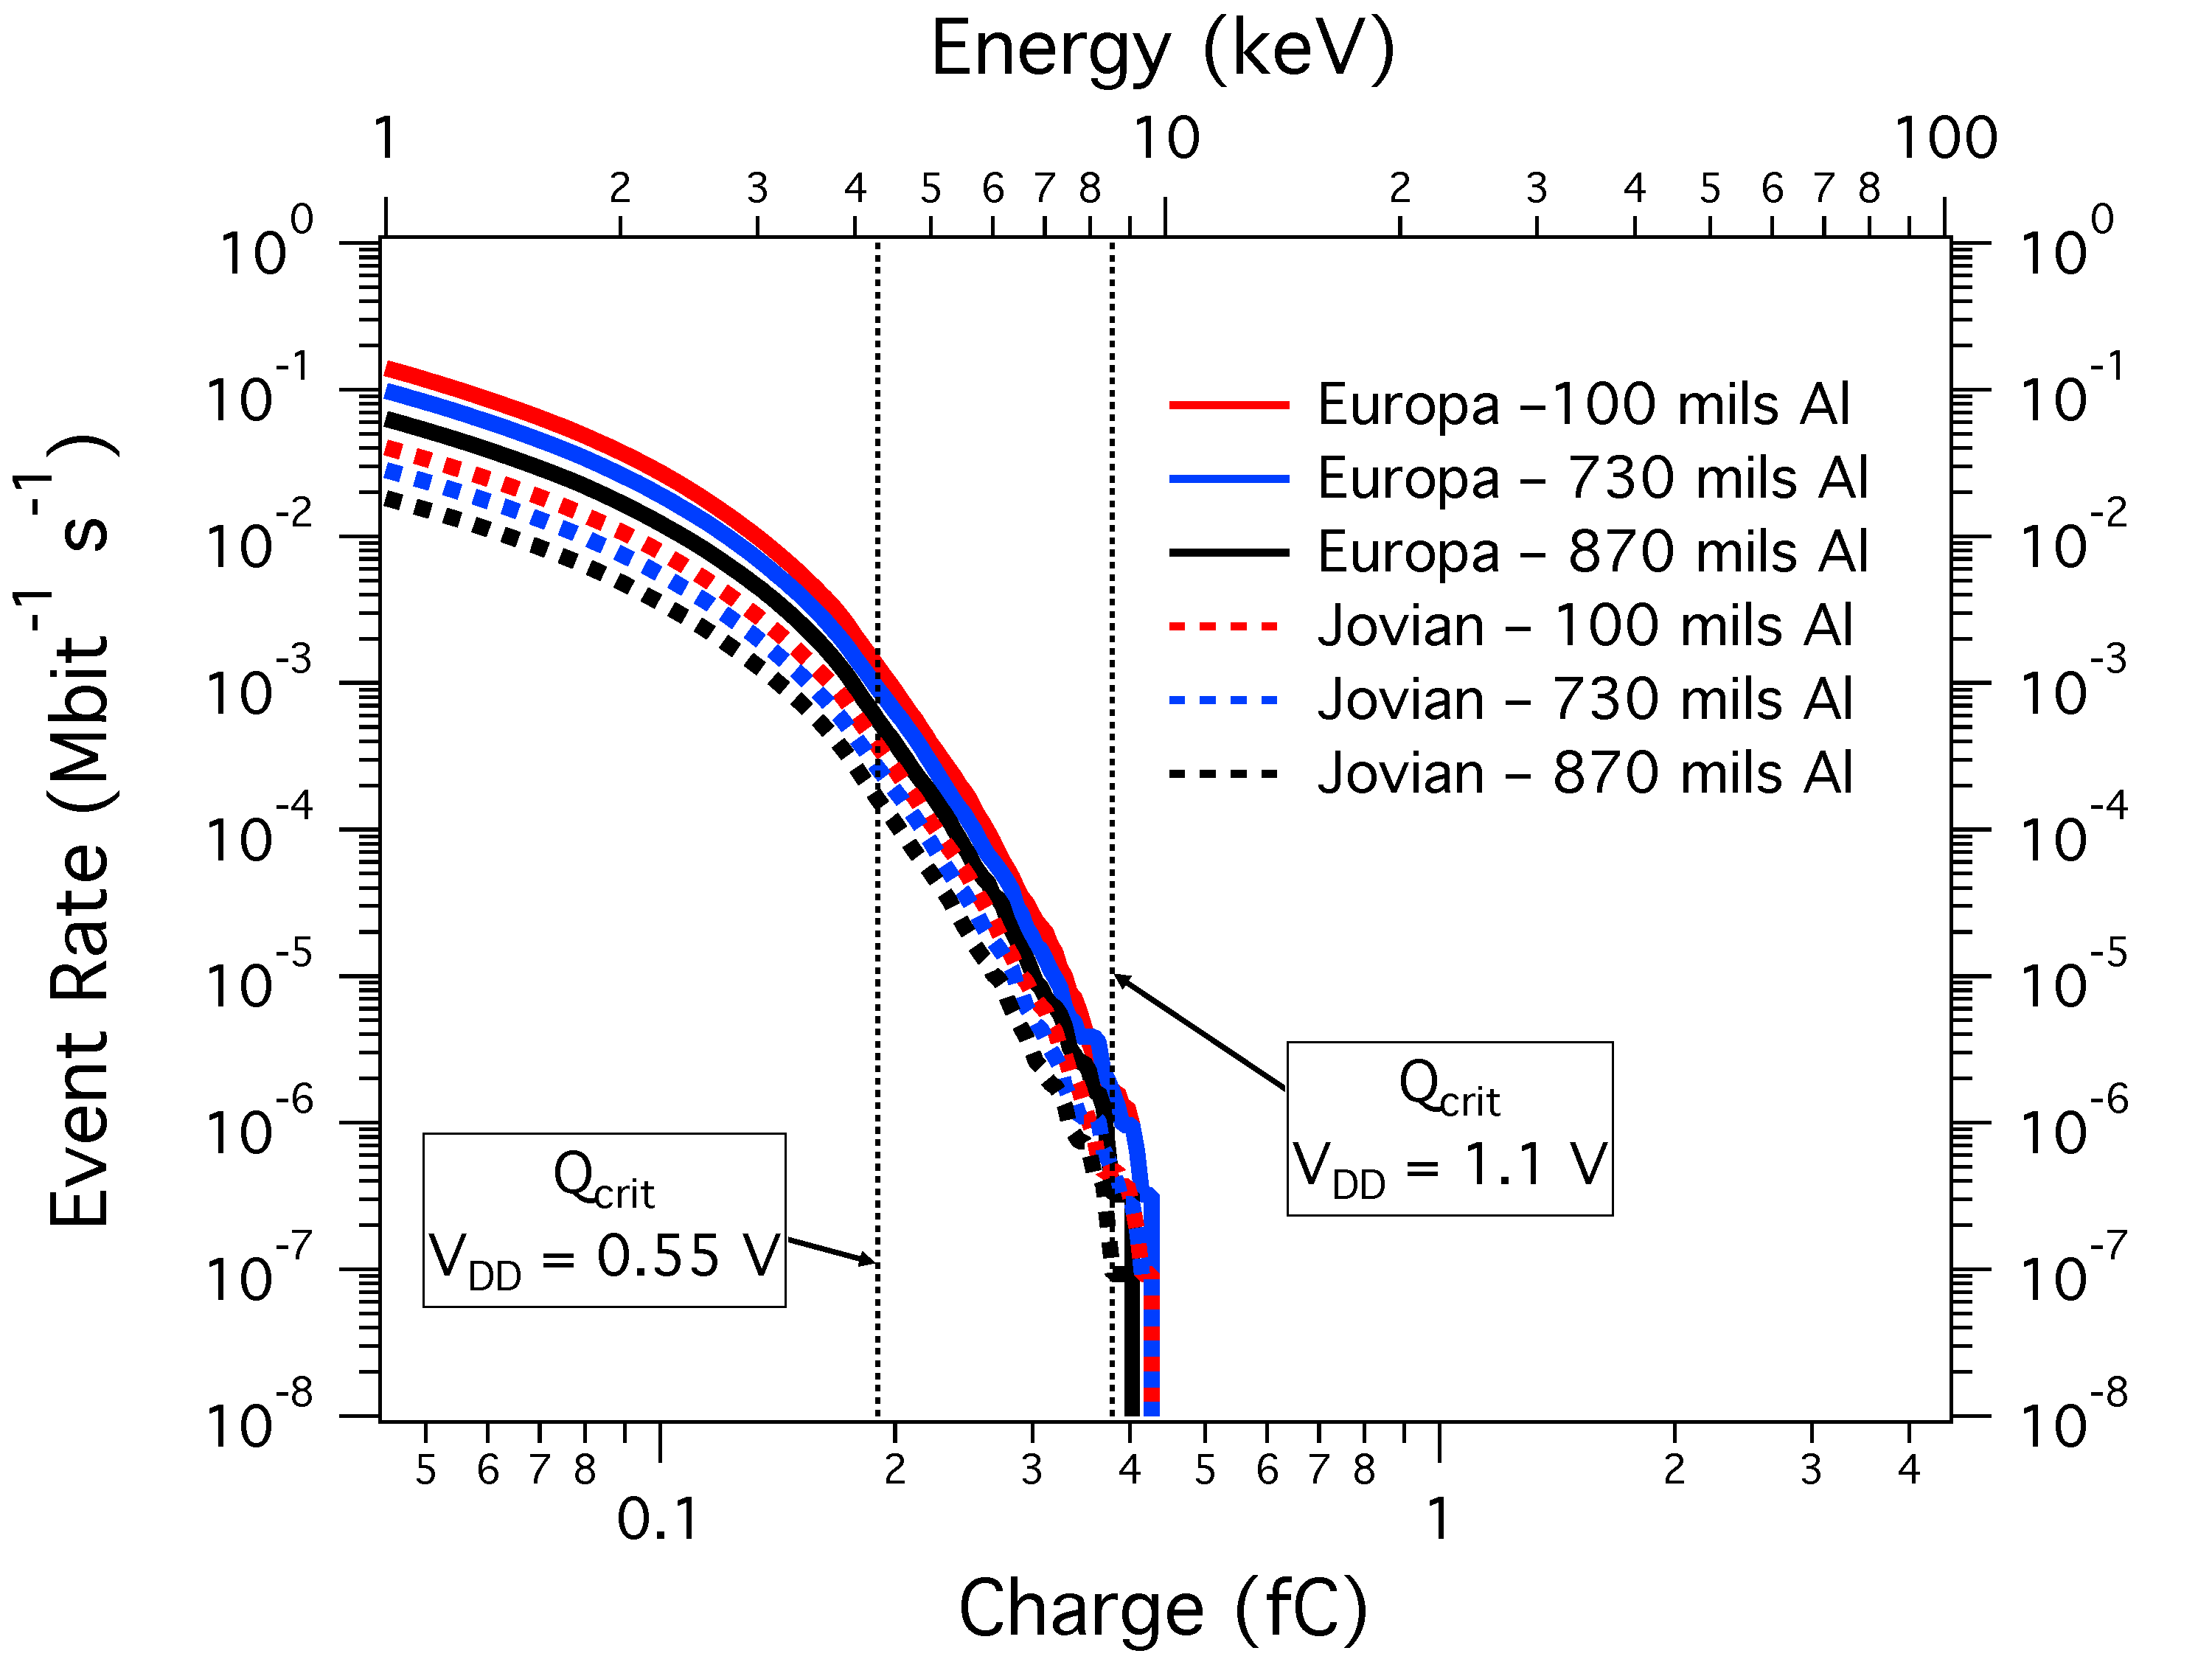
\includegraphics[width=6in]{europa-jovian-elec-rate-pred.pdf}
    \end{center}
    \caption{MRED simulations performed on the 45~nm structure from Fig.~\ref{fig:50kev_xrays_ppt} using the differential electron flux of Fig.~\ref{fig:jov-eur-elec-flux-env} for shielding thicknesses of 100, 730, and 870~mils of aluminum. 
    Results show that shielding has some impact on the overall electron-induced SEU error rate in the Jovian and Europa environments as shown by the slight reduction in event rates for equivalent orbits.
    Devices operated in a low-power or quiescent mode are likely to experience an unacceptably large upset rate while in proximity to the Jupiter planetary system.}
    \label{fig:europa-jovian-elec-rate-pred}
\end{figure}

\begin{figure}[htbp]
    \begin{center}
        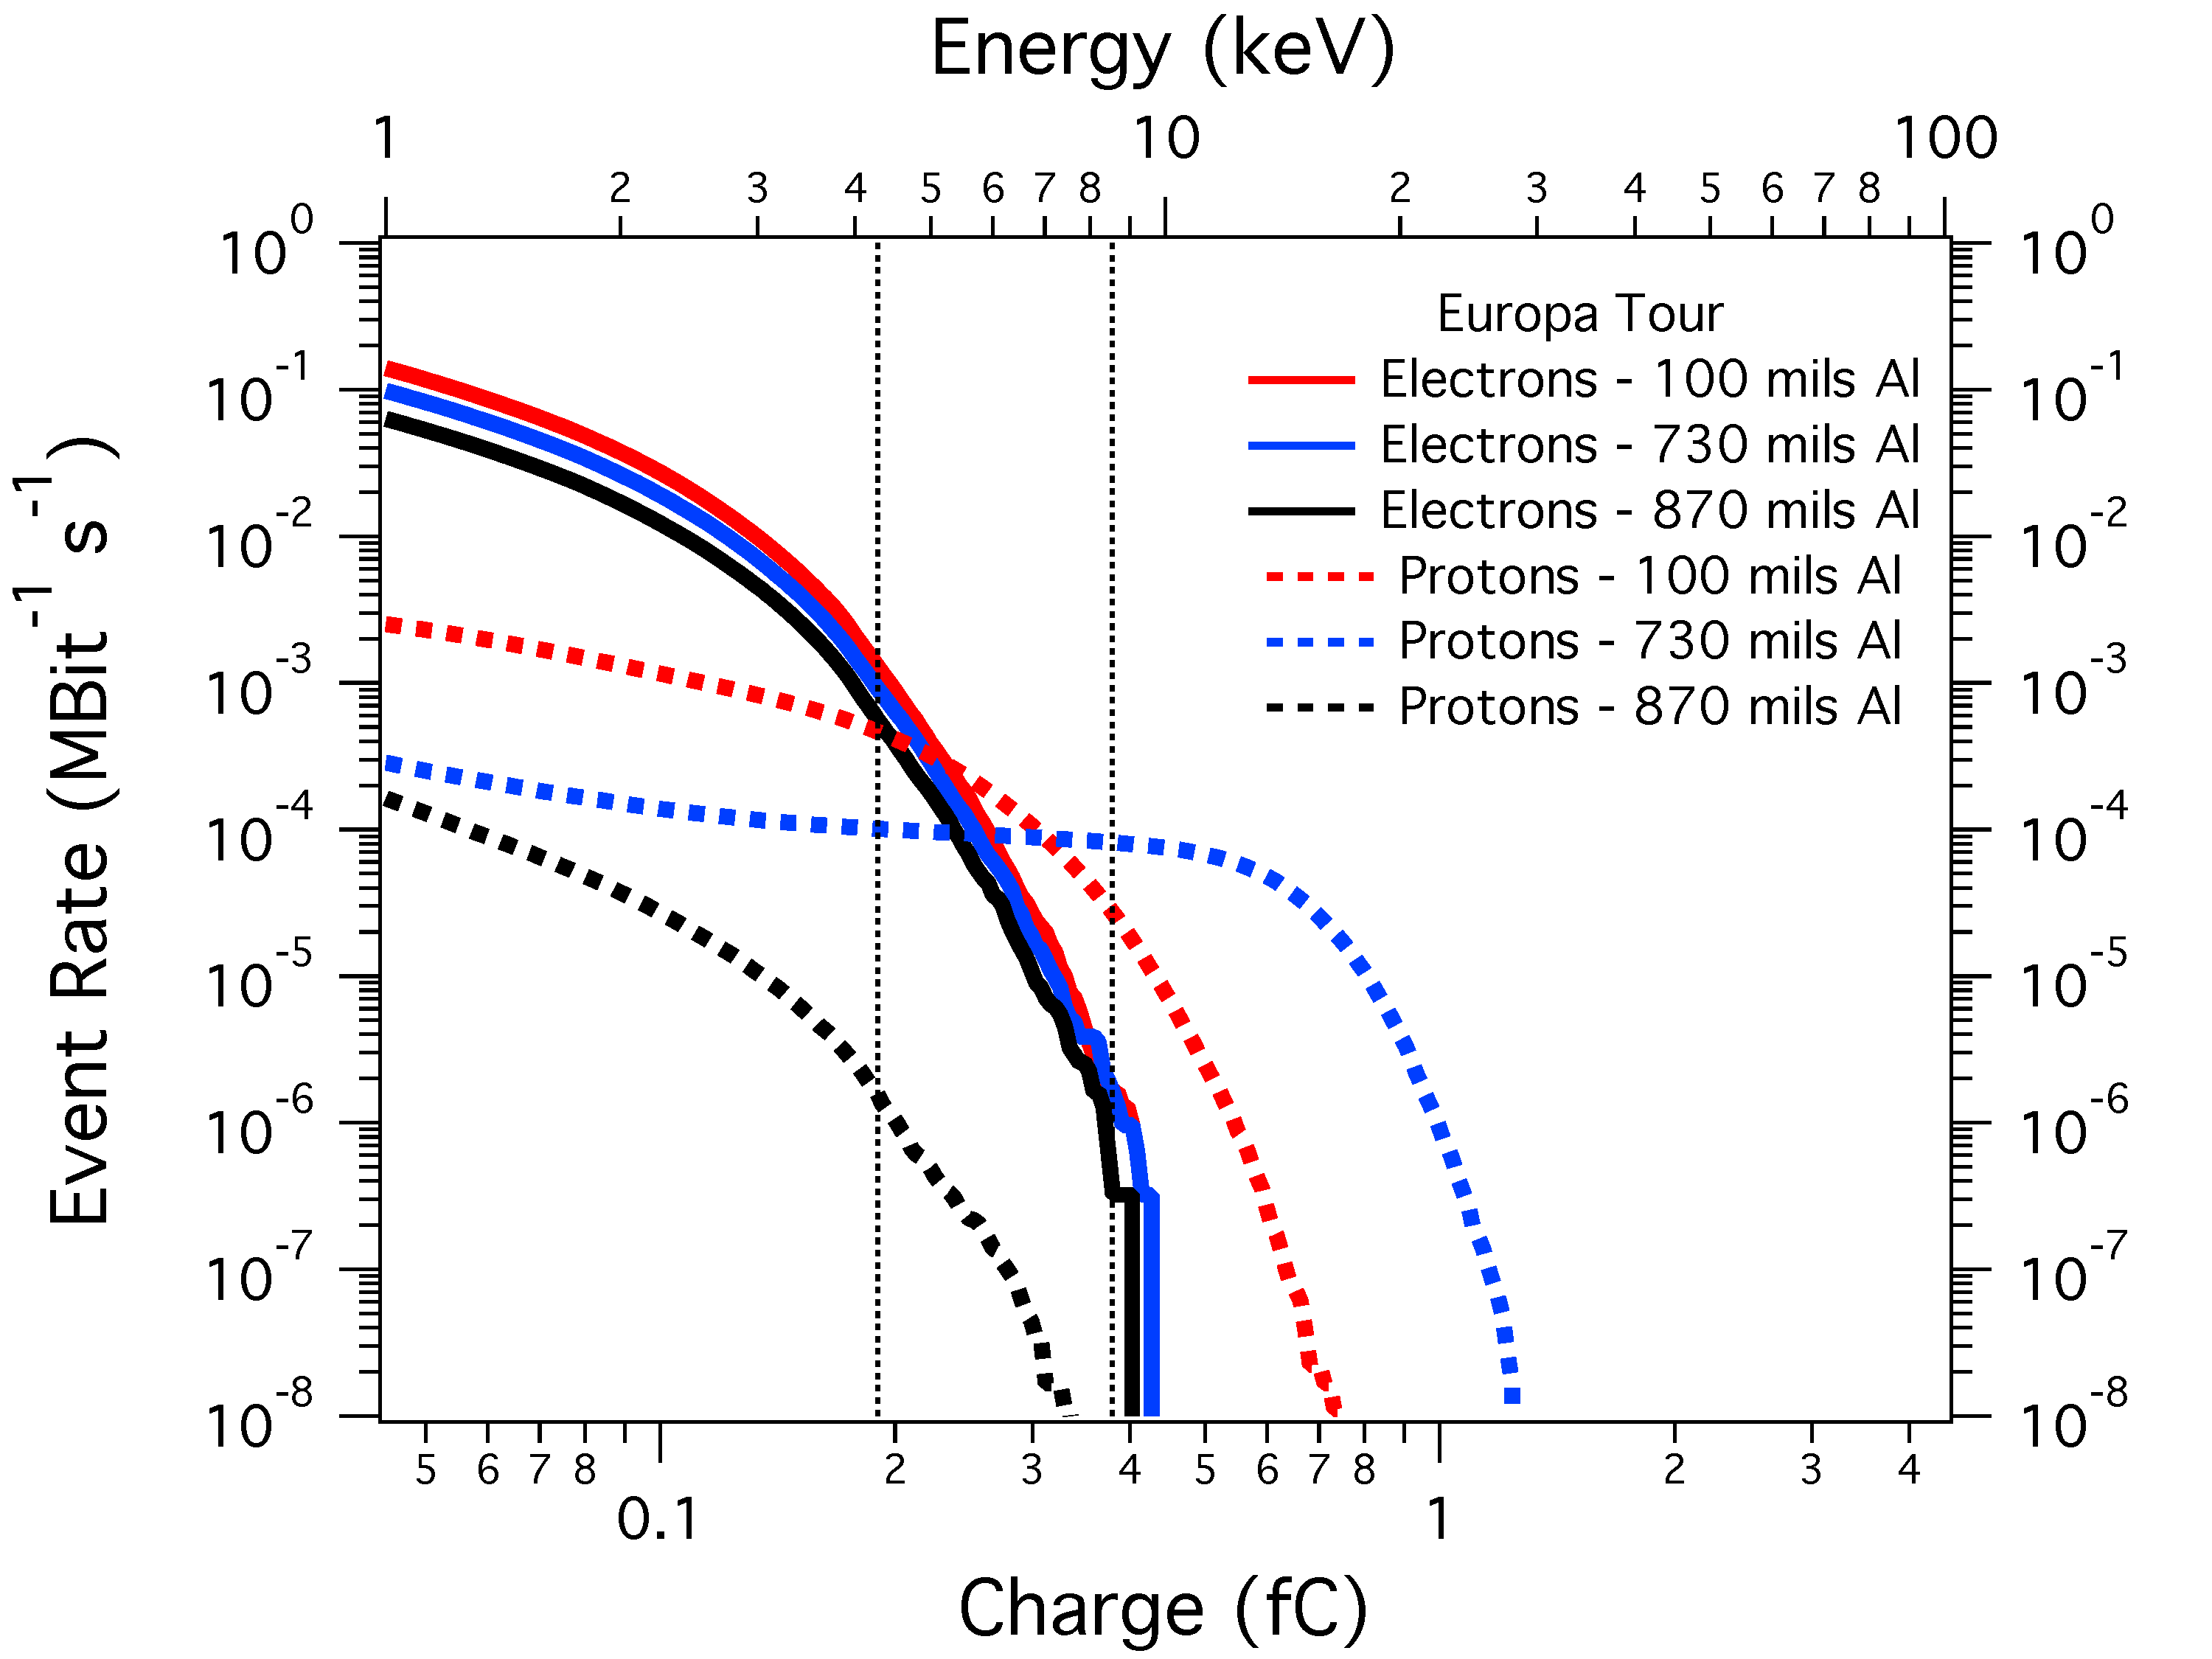
\includegraphics[width=6in]{europa-elec-prot-rate-pred.pdf}
    \end{center}
    \caption{MRED simulations performed on the 45~nm structure from Fig.~\ref{fig:50kev_xrays_ppt} using the electron environment of Fig.~\ref{fig:jov-eur-elec-flux-env} and proton environment of Fig.~\ref{fig:eur-prot-flux-env} for shielding thicknesses of 100, 730, and 870~mils of aluminum.
    Proton-induced SEU error rates are observed to be higher than electron-induced SEU error rates at nominal supply voltage. 
    Electron-induced SEU error rates become higher than proton-induced error rates under reduced bias conditions.
    }
    \label{fig:europa-elec-prot-rate-pred}
\end{figure}

Conclusions are similar for the Jovian trapped particle environment to those of the near-Earth when evaluating SEU error rate estimations.
Fig.~\ref{fig:europa-jovian-elec-rate-pred} shows the electron-induced SEU error rate as calculated by MRED simulations performed on the 45~nm structure from Fig.~\ref{fig:50kev_xrays_ppt} using the differential electron flux of Fig.~\ref{fig:jov-eur-elec-flux-env} for shielding thicknesses of 100, 730, and 870~mils of aluminum.
Results show that shielding has some impact on the overall electron-induced SEU error rate in the Jovian and Europa environments as shown by the slight reduction in event rates for equivalent orbits.
The difference in error rates for increasing shielding thicknesses appears to be negligible near nominal operating voltages for the 45~nm SRAM test chip while there is some indication that thicker shielding decreases the SEU error rate under reduced bias conditions.
Increasing shield thickness appears to provide diminishing returns for attenuating the electron-induced SEU error rate in near Juptier and Europa as it is impractical to use sufficient shielding to stop the 100~MeV electrons present in those environments.
The presence of higher energy electrons in the Europa electron flux spectrum does have an impact on the calculated error rates shown in Fig.~\ref{fig:europa-jovian-elec-rate-pred} as noted by their consistently higher event rates for all shielding thicknesses as compared to those of the Jovian environment.
Devices operated in a low-power or quiescent mode are likely to experience an unacceptably large upset rate while in proximity to the Jupiter planetary system.

Fig.~\ref{fig:europa-elec-prot-rate-pred} shows MRED simulations performed on the 45~nm structure from Fig.~\ref{fig:50kev_xrays_ppt} using the electron environment of Fig.~\ref{fig:jov-eur-elec-flux-env} and proton environment of Fig.~\ref{fig:eur-prot-flux-env} for shielding thicknesses of 100, 730, and 870~mils of aluminum.
Proton-induced SEU error rates are observed to be higher than electron-induced SEU error rates at nominal supply voltage conditions. 
While the proton flux is significantly attenuated by the presence of the aluminum shielding, this results in a proton spectrum that is more likely to cause bit-flips within the SRAM cell.
This is shown by the slight increase in event rate for shielding thicknesses of 730 and 870~mils as compared to that of 100~mils.
Interestingly, Fig.~\ref{fig:europa-elec-prot-rate-pred} suggests that electron-induced SEU error rates are estimated to be higher than proton-induced error rates under reduced bias conditions.
This is very similar to trends observed in Figs.~\ref{fig:28nm_xray_muon_proton} and \ref{fig:45nm_xray_muon_proton} where the measured SEU cross-section for protons was higher than that of electrons near nominal supply voltage conditions.
However, as supply voltage decreases, the electron-induced SEUs cross-section increased at a much higher rate than the proton cross-sections and could potentially lead to a higher measured cross-section at reduced bias conditions.

Comparing the electron-induced SEU error rates for the near-Earth and Jovian environments yields fairly consistent results.
Although the environments are dramatically different, the calculated SEU error rates suggest that electron-indued SEUs at or near nominal bias conditions are extremely rare events and unlikely to contribute significantly to error rates in SRAMs fabricated in current sub-65~nm technology nodes.
The presence of high fluxes of energetic electrons, as high as 100~MeV, has a significant impact on error rates, especially under reduced bias conditions, in the Jovian environment when compared to that of the lower energy electrons found in the Van Allen radiation belts.
The differences between the Jovian and near-Earth environments is most significant at reduced bias conditions where electron-induced SEU error rates are higher than those of the geosynchronous environment by more than an order of magnitude.
Furthermore, the estimated error rates in Figs.~\ref{fig:geo_max_rate_pred_ae8_ppt} and \ref{fig:europa-jovian-elec-rate-pred} suggest that spacecraft operating near an enegertic electron environment, like those found in the Van Allen radiaiton belts or the Jupiter planetary system, that enter into a power-saving or quiescent mode would significantly increase the likelihood of SEUs contributing to anomalous behavior in the onboard electronics systems.
% section electron_induced_seu_event_rates (end)

\section{Impact of Delta-rays on Microelectronics} % (fold)
\label{sec:impact_of_delta_rays_on_microelectronics}
In this section, single ionizing particles are simulated.
The resulting tracks are analyzed, and energy deposited by $\delta$-rays within small volumes is evaluated as a function of position within a large silicon structure.
The evaluation volumes are 50~nm cubes, representing regions where energy deposition results in the generation and collection of charge that contributes to the device response.

The sensitive volume model and approach for evaluating upset events in SOI used in this section is consistent with \cite{King:2010jg,King:2012cb,Haran:2008ve}.
The sensitive volumes are 50~nm cubes that are representative of typical active regions in modern SOI technology \cite{Haran:2008ve}. 
A concentric cylindrical target of silicon is utilized to characterize the radial dependence of energy deposition from the incident ion track structure; the thickness of the target structure is 50 $\mu$m. 
The range of all incident particles evaluated in this section is much longer than the thickness of the target. 
The threshold for an upset event is defined as in previous sections, the amount of energy deposited in the sensitive volume required to generate the device’s critical charge.
IBM has reported their 65~nm SOI technology node to have a critical charge between 0.14-0.28~fC \cite{Rodbell:2007vl}, which corresponds to energy deposition of 3.15-6.3~keV within the sensitive volume. 
Additionally, the critical charge estimate of 0.08~fC for upset from \cite{King:2010jg} corresponds to 1.8~keV of energy deposited within the sensitive volume and is used to evaluate the sensitivity of future technology nodes. 
It is assumed that energy below this threshold does not result in an upset event, and energy deposition greater than or equal to the threshold results in an upset.

Events are simulated using He and Ne ions; the energy 
distribution of $\delta$-rays generated will be similar for fixed  
incident ion energy, their generation rate will depend on the incident ion
LET.
The target geometry is chosen to be cylindrically symmetric about the incident ion path, energy deposition is evaluated as a function of orthogonal distance from the trajectory of the incident ion. 
The energy deposited within a 50~nm cube is sorted by the orthogonal distance from the incident ion trajectory and the magnitude of energy deposited.
The resulting histograms are described by a function $f(E,R)$ which represents the differential energy spectrum in a 50~nm cube at radius $R$.

Using this method, the sensitive volumes generated consistently account for the largest energy deposited by the ensemble of $\delta$-rays in a local region of target material during a simulated heavy-ion event. 
Consequently, this calculation represents a worst-case analysis of ``track structure'' contributions to SEUs. 
The representation of a 560~MeV~N event using this technique can be seen in Fig.~\ref{fig:560_MeV_N_track}.
\begin{figure}[tb]
     \begin{center}
         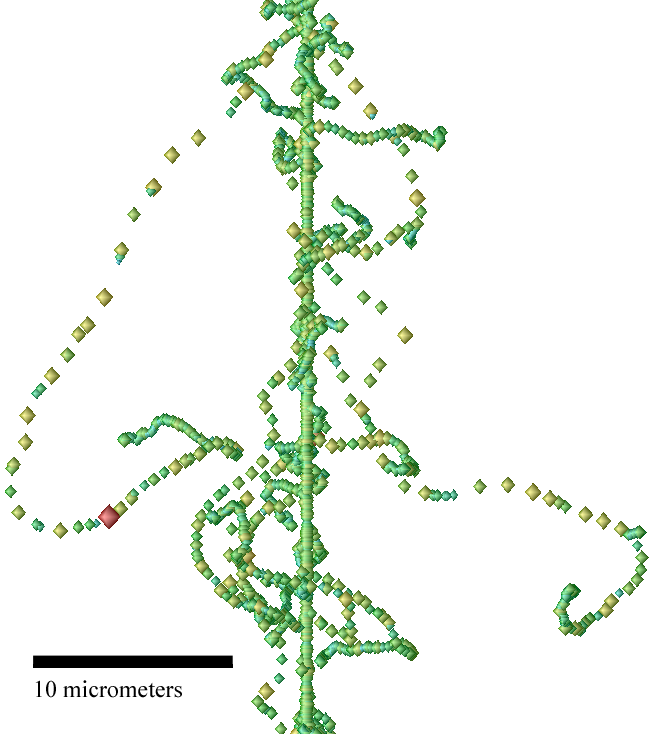
\includegraphics[height=5.5in]{560MeVN_track_2_copy_final.png}
     \end{center}
     \caption{Representation of a the energy deposition from $\delta$-rays generated by a single 560~MeV~N ion incident on a large silicon structure. Each box represents the energy deposited by $\delta$-rays in a specific region. The magnitude of energy deposited at each location is represented as color intensity, where warmer colors are larger energy deposition events.}
     \label{fig:560_MeV_N_track}
 \end{figure} 
Each cube represents the location of energy deposited by $\delta$-ray(s) and illustrates the spatial non-uniformity and variation in magnitude of $\delta$-ray energy deposition events along their trajectory. 
The color intensity scale shows the magnitude of energy deposited, where warmer colors, red for example, represent larger energy deposition events and cooler colors, such as green, represent smaller energy deposition. 
This allows the visual representation of heavy-ion track structure and identification of the spatial location of large energy deposition events.

\begin{figure}[tb]
    \begin{centering}
        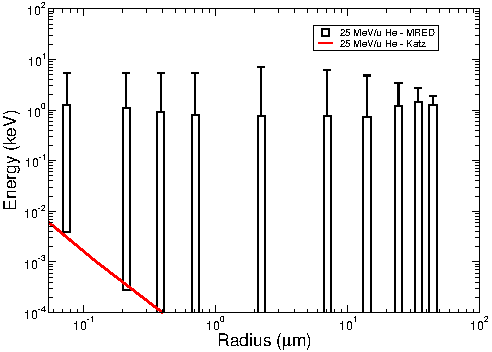
\includegraphics[width=5in]
        {25_MeVpU_He_energyDist_vs_katz-eps-converted-to.pdf}
        \caption{
        Simulation results show good agreement for energy deposited within a 50~nm cube by the Katz model (solid red line) and MRED for 25 MeV/u~He. The lower edge of the box is the average energy, the upper edge of the box is the 90th percentile event, and the whisker is the largest energy deposition event. While the average energy within a 50~nm cube shows a strong dependence on the radial distance, MRED shows that large energy deposition events occur at radial distances greater than 10~$\mu$m.
        }
        \label{fig:katzComp25MeVuHe}
    \end{centering}
\end{figure}
\begin{figure}[hbtp]
    \begin{centering}
        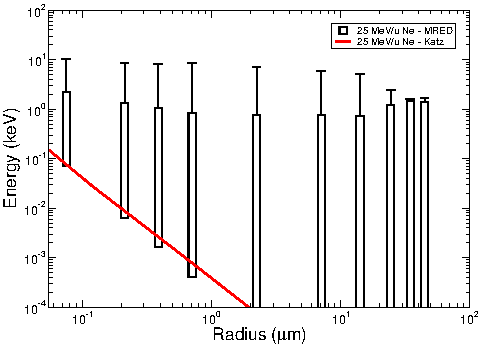
\includegraphics[width=5in]
        {25_MeVpU_Ne_energyDist_vs_katz-eps-converted-to.pdf}
        \caption{
        Simulation results show good agreement for energy deposited within a 50~nm cube by the Katz model (solid red line) and MRED for 25 MeV/u~Ne. The lower edge of the box is the average energy, the upper edge of the box is the 90th percentile event, and the whisker is the largest energy deposition event. Large energy deposition events are again shown to occur at radial distances larger than 10~$\mu$m.
        }
        \label{fig:katzComp25MeVuNe}
    \end{centering}
\end{figure}

Figs.~\ref{fig:katzComp25MeVuHe} and \ref{fig:katzComp25MeVuNe} compare the energy deposited within a 50~nm cube for the analytical expectation of the Katz model,\cite{Chunxiang:1985uo, Fageeha:1994tc} shown as the solid red line, with results obtained using MRED, represented by the box and whisker data set in black.
MRED data represents the average energy within a 50~nm cube, shown as the lower edge of the box, the 90th percentile of events, shown as the upper edge of the box, and the whisker, representing the largest energy deposition event observed.
Simulation results indicate that MRED agrees well with the Katz model expectation of energy within a 50~nm cube as shown by the lower edge of each box and the red line.
The Katz model expectation represents the total energy deposited within a cylindrical shell for a single ion event.
Figs.~\ref{fig:katzComp25MeVuHe} and \ref{fig:katzComp25MeVuNe} demonstrate that the Katz model contains no information regarding the frequency or magnitude of individual energy deposition events involving $\delta$-rays.
Individual scattering events may deposit significantly more energy within a 50~nm cube than the average would predict, as illustrated by the 90th percentile and extreme values shown in Figs.~\ref{fig:katzComp25MeVuHe} and \ref{fig:katzComp25MeVuNe}.
Information regarding the magnitude of energy deposited and spatial resolution of individual $\delta$-ray scattering events is lost when averaging the total energy deposited in large volumes, as in the Katz model.

MRED indicates that $\delta$-ray scattering events can deposit up to 10~keV of energy within a 50~nm cube at radial distances tens of micrometers away from the incident ion trajectory.
By contrast, the average energy obtained from Katz model is less than 3.6~eV, the average energy required to produce a single \emph{eh} pair in silicon, after several hundred nanometers for both 25~MeV/u~He and Ne.
Under-predicting the magnitude of energy deposited results in inaccurate charge generation and collection profiles.
Scaling the expected energy deposition obtained using the Katz model into small volumes introduces error and results in inaccurate conditions for evaluating the device response.
Figs.~\ref{fig:katzComp25MeVuHe} and \ref{fig:katzComp25MeVuNe} demonstrate that MRED captures a level of detail greater than the Katz model provides, allowing further analysis of $\delta$-ray events and their impact on device response.

Events occurring more than 25~$\mu$m from the incident ion trajectory
are near the maximum range of $\delta$-rays generated by 25~MeV/u He 
and Ne and occur with a frequency up to six orders of magnitude lower 
than those of events at smaller radial distances.
Fifty micrometers is therefore used as the evaluation limit in these simulations.
The $\delta$-rays involved in energy deposition events at radial
distances greater than 25~$\mu$m are near their stopping range, 
which results in
a reduction in the maximum energy deposition event and increase in 
the 90th percentile event as seen in Figs.~\ref{fig:katzComp25MeVuHe}
and \ref{fig:katzComp25MeVuNe}.

 The differential energy spectrum $f(E,R)$ is represented as a cumulative energy distribution by the expression
\begin{equation}
    \label{eq:cumDistFx}
    \frac{d}{dx}F(E_i, R) = \frac{1}{\theta(R) N} \frac{l_{cube}}{x} \sum_{j \ge i}^{\infty} f(E_i,R)
\end{equation}
where $R$ is the orthogonal distance from the incident particle trajectory, $N$ is the number of incident particles evaluated, $l_{cube}$ is the side length of an evaluation volume parallel to the z-axis, $x$ is the ion path length through the target material, $\theta(R)$ is the (one-dimensional) solid angle subtended by a cubic volume at an orthogonal distance $R$ from the incident particle trajectory, and $f(E,R)$ is the differential energy distribution.
The formulation of Eq.~\ref{eq:cumDistFx} for a single ionizing particle event represents the probability per radian of observing a $\delta$-ray energy deposition event greater than or equal to $E_i$.
Equivalently, Eq.~\ref{eq:cumDistFx} represents the probability of a single ionizing particle event depositing a given amount of energy, $E_i$, or more within a cube with dimensions $l_{cube}$ at a distance $R$.
Normalizing to the thickness of the evaluation volume, $l_{cube}$, and total thickness of the target material, $x$, reduces the problem to a two dimensional space in the plane normal (the $y-z$ plane) to the incident ion trajectory.
Because the target geometry is cylindrically symmetric about the incident ion path, normalizing to the angle $\theta$ allows a direct comparison of the probability to observe events of a given energy magnitude or greater at different radial distances from the incident ion trajectory. 

From this, relationships about the frequency of $\delta$-ray events at different radial distances can be inferred.
When Eq.~\ref{eq:cumDistFx} evaluates close to unity, this implies a high likelihood of observing an event of a given magnitude within a geometric volume at a particular distance.
A reduction in the frequency of events with increasing distance indicates the termination of $\delta$-ray trajectories.

\begin{figure}[tb]
    \begin{centering}
        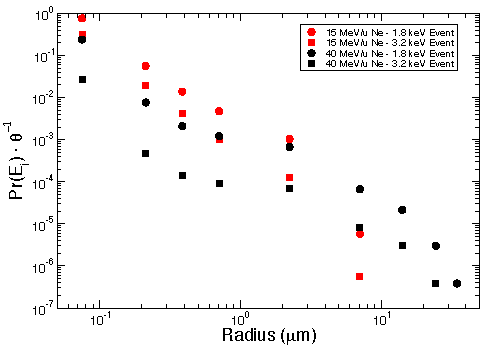
\includegraphics[width=5in]
        {prob_comp_apl_fig3_ap.pdf}
        \caption{
            Cumulative energy distribution as a function of radial distance for 15~MeV/u and 40~MeV/u Ne ions. Results show the frequency of $\delta$-ray energy deposition events depend on LET and energy of the incident particle.
        }
        \label{fig:LETandEnergyDep}
    \end{centering}
\end{figure}

Fig.~\ref{fig:LETandEnergyDep} plots the cumulative energy distribution calculated by Eq.~\ref{eq:cumDistFx} as a function of radial distance for one thousand simulated particle events. 
Data points are plotted for energy deposition events greater than or equal to 1.8~keV and 3.2~keV within a 50~nm cube for 15~MeV/u and 40 MeV/u Ne.
These incident ion energies are representative of several energy tunes available at the TAMU cyclotron facility.
The corresponding LETs are 2.6~MeV$\cdot$cm$^2$/mg and 1.2~MeV$\cdot$cm$^2$/mg, respectively.
Scattering and stopping of $\delta$-rays is evident in Fig.~\ref{fig:LETandEnergyDep} due to the construction of Eq.~\ref{eq:cumDistFx} and is shown by the decreasing probability of events with increasing distance. 
Fig.~\ref{fig:LETandEnergyDep} also indicates that smaller energy deposition events occur much more frequently than larger energy deposition events as shown by the 1.8~keV curves compared to the 3.2~keV curves.
The relationships shown in Fig.~\ref{fig:LETandEnergyDep} also show that while large energy deposition events, on the order of 1~keV or more, may occur at radial distances tens of micrometers from an incident ion path, as indicated in Figs.~\ref{fig:katzComp25MeVuHe} and \ref{fig:katzComp25MeVuNe}, the likelihood of such events occurring decreases with increasing distance from the incident ion path.

This suggests that the regions mostly likely to be affected by $\delta$-rays in a single ionizing particle event are likely to occur within five micrometers surrounding the incident ion strike location, the distance at which the likelihood of an event depositing sufficient energy to exceed the estimated critical charge of a 22~nm SRAM falls below $Pr(E_i) = 10^{-6}$.

Fig.~\ref{fig:LETandEnergyDep} also illustrates the role of incident ion LET and energy in $\delta$-ray events.
 At radii near the incident ion trajectory, higher LET particles have a higher probability of depositing large amounts of energy than lower LET particles.
 This is easily observed in the relative frequency of 1.8~keV energy deposition events for 15~MeV/u~Ne compared to 40~MeV/u~Ne.
 This is due primarily to the generation of many low-energy, short-range $\delta$-rays depositing energy around the incident ion's trajectory.
 The maximum transferable energy from Eq.~\ref{eq:emax} limits the radial extent of the ion track radius, as shown by decreasing probability of energy deposition events with increasing distance from the incident ion trajectory.
 Consequently, higher energy incident particles can produce undesirable effects in microelectronics at larger radial distances and with greater frequency than lower energy ions.

 Monte-Carlo simulation results indicate that in technology nodes where less than 0.5~fC of charge result in circuit-level effects, $\delta$-rays may contribute to the upset error rate.
 A comparison of MRED with the Katz model demonstrates average track structure models alone are inadequate in capturing the device response.
 The probability of $\delta$-ray related effects exhibits a strong dependence on both incident ion energy and LET.
 Additionally, the likelihood of $\delta$-ray induced effects exhibits a strong dependence on radial distance from the incident ion path.
 
 These results have strong implications for ground-based parts qualification testing and space radiation environments, where varying incident ion energy and LET result in differing contributions from $\delta$-rays to device and circuit level effects.
% section impact_of_delta_rays_on_microelectronics (end)
% chapter simulation_of_electron_induced_seus (end)